\chapter{激进的极大二分团枚举剪枝方法}
\label{ch:aggressive_mbe}

针对极大二分团枚举问题搜索空间大、现有剪枝方法效率低下的问题,本章整理了相关工作中的优化方法,并指出其中的共性问题作为本章的研究动机。具体而言,我们发现通用的集合枚举树存在结构限制,即仅允许利用部分顶点生成新的枚举节点,导致产生大量包含非极大二分团的无效枚举节点;同时,已有的剪枝方法仅在当前节点通过节点检查后被动执行,剪枝效率受限。为解决这些问题,本章提出了以下优化方法:首先,针对集合枚举树的结构限制,本章提出了激进的集合枚举树。该枚举树激进地将枚举树中每个节点对应的二分团扩展为极大二分团,并利用父子节点间的联系消除枚举树中的重复二分团,从而低成本裁剪无效节点且保持树结构平衡。然后,针对现有方法被动触发的特点,本章提出了激进的顶点合并剪枝方法。该方法主动地合并具有相同局部邻居的顶点,进一步提升了剪枝效率。最后,本章结合激进的集合枚举树和激进的顶点合并剪枝方法,形成了高效的极大二分团枚举算法AMBEA。实验证明,AMBEA算法相比现有最优算法压缩了2.37-8.98倍的搜索空间,运行时间缩短了1.15-5.32倍。

\section{现有搜索空间优化方法分析}
\label{sec:opt}

为了优化极大二分团枚举问题的搜索空间,相关工作以~\ref{subsec:baseline}节所述的集合枚举树为基础,设计了许多优化方法。本节将这些方法总结为三类:顶点排序方法、基于枢纽顶点的剪枝方法和被动的顶点合并剪枝方法。本节将对这些方法进行详细说明。

\subsection{顶点排序方法}
\label{subsec:order}

顶点排序方法是一种常用的搜索空间优化技术,在枚举领域中得到了广泛应用。以极大团枚举问题为例,Eppstein等人提出了退化排序方法~\cite{MCEdegeneracy10}。该方法根据当前顶点与未选取顶点的连接关系进行排序,将连接度低的顶点放在前面,以此限制每个枚举节点内候选顶点数量的上限来降低算法的最坏时间复杂度,从而压缩问题的搜索空间。虽然顶点排序会增加排序的开销,但是好的顶点排序方法可以显著地减小搜索空间,从而提高整体性能。因此,在近些年,研究者们广泛采用退化排序方法来解决极大团枚举问题~\cite{MCEparallel20,MCE20,MCE22,MCE-GPU21,MCE-22}和最大团搜索问题~\cite{MEC20,MEC22}。


% 顶点排序方法是一种常用的搜索空间优化技术,在枚举领域中得到了广泛应用。以极大团枚举问题为例,Eppstein等人提出了退化排序方法~\cite{MCEdegeneracy10}。该方法在选择下一个顶点时考虑了之前已选取的顶点与未选取的顶点之间的连接关系,并通过限制每个枚举节点内候选顶点数量的上限来降低算法的最坏时间复杂度,从而压缩问题的搜索空间。虽然顶点排序会增加排序的开销,但是好的顶点排序方法可以显著地减小搜索空间,从而提高整体性能。因此,在近些年,研究者们广泛采用退化排序方法来解决极大团枚举问题~\cite{MCEparallel20,MCE20,MCE22,MCE-GPU21,MCE-22}和最大团搜索问题~\cite{MEC20,MEC22}。



% 如图~\ref{fig:order_inc}和图~\ref{fig:order_dec}所示,对于一个仅包含5个极大二分团的二分图$G_0$,不同的排序方法产生非极大二分团数量是不一样的,即对应的搜索空间是不同的。



在极大二分团枚举问题中,顶点排序方法同样适用。根据节点的生成规则,每个节点$(L,R,C)$可以按照任意顺序遍历候选顶点集$C$中的顶点生成新的节点$(L',R',C')$。由于在枚举过程中,集合$C$是二分图$G(U,V,E)$中集合$V$的子集,因此极大二分团枚举问题中的顶点排序默认只对集合$V$中的顶点进行排序。基于这一理论基础,研究者们设计了多种不同的顶点排序方法。
% 通过对比图~\ref{fig:order_inc}和图~\ref{fig:order_dec},我们可以观察到
不同的顶点遍历顺序会导致产生的非极大二分团数量有所差异,相应的搜索空间大小也不同。与退化排序方法在极大团枚举问题中的地位不同,在极大二分团枚举问题中,不同的顶点排序方法各具优势。以下是对这些排序方法的梳理。

(1)根据顶点的邻居数量递增排序。在频繁项集挖掘领域中,根据邻居数量对顶点进行递增排序的方法被广泛采用,并且实践证明这种方法对搜索空间的优化非常有效~\cite{lcm04}。采用这种排序方法可以使得邻居数量较少的顶点拥有较多的尾部顶点,即$|N(v)|$越小,$|X_v^+|$越大。结合集合枚举树的节点生成规则,我们可以推导出在这种排序条件下,邻居较少的顶点对应的子搜索空间受到顶点数量的约束;而邻居较多的顶点对应的子空间受到尾部顶点数量的约束,从而提供性能保障。因此,大量的极大二分团枚举相关工作采用这种排序方式~\cite{lcmmbc07,minel06,iMBEA14,mapreduceMBE16,parMBE19,MEB20},代表算法包括MineLMBC~\cite{minel06},iMBEA~\cite{iMBEA14},FMBE以及它的并行版本ParMBE~\cite{parMBE19}。此外,MineLMBC和iMBEA算法也会按照局部邻居的数量递增对每个节点$(L,R,C)$内的候选顶点进行排序,即对集合$C$内的顶点$v$根据$|N_L(v)|$的大小递增排列。但需要注意的是,这种排序方式会增加每个节点的计算量,因此需要在平衡排序开销和带来的性能收益方面进行考虑。

(2)根据顶点的邻居数量递减排序。在真实的二分图场景下,很多二分图的顶点邻居数量分布呈现出倾斜的特征。Damaschke的研究表明,如果顶点邻居数量的分布符合齐夫定律(Zipf's law),那么按照顶点邻居数量递减排序可以降低极大二分团枚举算法的最坏时间复杂度~\cite{Damaschke14}。然而,实际情况中很多二分图并不能完全满足这种严格的分布约束。此外,Damaschke的研究主要关注优化算法的最坏时间复杂度。
鉴于该时间复杂度相对较为宽松,因此不能准确反映极大二分团枚举任务的实际运行时间。
% 由于这个时间复杂度是相对宽松的,因此它并不能准确反映极大二分团枚举任务的实际运行时间。


(3)逆拓扑排序。在Abidi等人的研究中,他们发现二分图中顶点邻居的包含关系可以用来裁剪搜索空间中的非极大二分团~\cite{PMBE20}。举个例子,如果对于两个顶点$v_1$和$v_2$,$v_1$的邻居集合包含$v_2$的邻居集合 (即$N(v_1)\supset N(v_2)$),那么所有包含顶点$v_2$且不包含$v_1$的二分团都是非极大二分团,可以进行剪枝。基于这个思想,Abidi等人设计了基于枢纽的顶点剪枝方法,并设计了逆拓扑排序来辅助进行枢纽顶点的选择。具体来说,他们根据二分图中顶点邻居的包含关系构建有向图CDAG。如果$N(v_1)\supset N(v_2)$,则在CDAG中添加一条有向边$v_1\rightarrow v_2$。最终,根据CDAG对顶点进行逆拓扑排序。目前,该排序方法仅在PMBE算法中使用~\cite{PMBE20}。

(4)单边排序。Chen等人结合极大团枚举问题中的退化排序方法~\cite{MCEdegeneracy10}和二分图的特征提出了单边排序方法。考虑到极大二分团枚举问题中候选顶点的数量取决于顶点的二跳邻居数量,单边排序根据当前顶点在未选取顶点中的二跳邻居数量进行排序,将二跳邻居数量较少的顶点排在前面。类似于根据顶点邻居数量递增排序的思路,这种排序方法可以使得二跳邻居数量较少的顶点能够拥有更多的尾部候选顶点。因此我们知道,二跳邻居数量较少的顶点对应的子搜索空间受到顶点二跳邻居数量的约束;而二跳邻居较多的顶点对应的子空间受到尾部顶点数量的约束,从而限制每个枚举节点内候选顶点数量的上限,压缩问题的搜索空间。目前,该排序方法仅在ooMBEA算法中使用~\cite{ooMBE22}。

% (4)单边排序。Chen等人结合极大团枚举问题中的退化排序方法~\cite{MCEdegeneracy10}和二分图的特征提出了单边排序方法。该方法根据当前顶点在未选取顶点中的二跳邻居数量进行排序,将二跳邻居数量较少的顶点放在前面,以此限制每个枚举节点内候选顶点数量的上限来降低算法的最坏时间复杂度,从而压缩问题的搜索空间。目前,该排序方法仅在ooMBEA算法中使用~\cite{ooMBE22}。

总体而言,在极大二分团枚举问题中,顶点排序方法的选择是灵活的,并且其性能取决于它与对应算法的配合程度。例如,逆拓扑排序方法可以辅助PMBE算法选择枢纽顶点,而其他排序方法不具备这种效果。因此,研究者们需要结合具体的枚举算法来选择合适的顶点排序方法。


接下来,我们将通过一个具体例子来说明顶点排序方法在极大二分团枚举问题中的实际效果:

\begin{figure} [H]
  \center
    % \vspace{0.1in}
		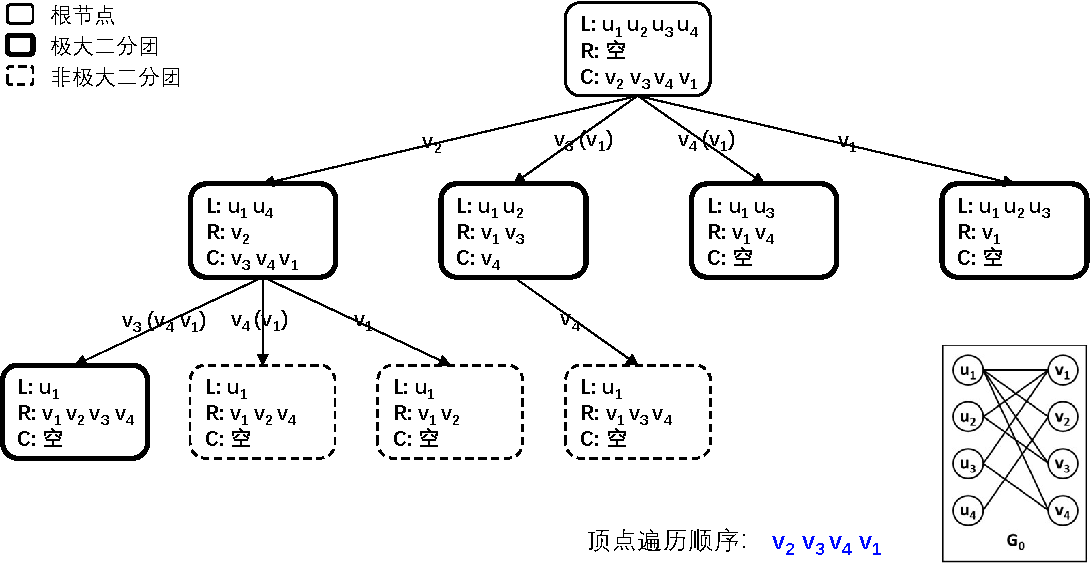
\includegraphics[width=0.8\linewidth]{order_inc}
    % \vspace{0.05in}
	\caption{根据顶点的邻居数量递增排序}
	\label{fig:order_inc}
\end{figure}


\begin{figure} [H]
  \center
  \vspace{0.1in}
    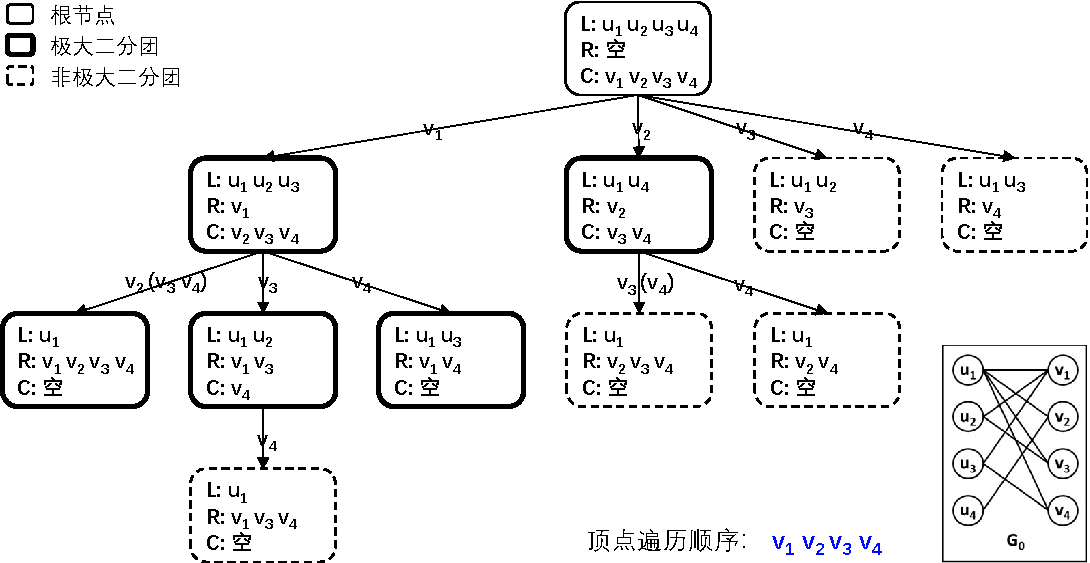
\includegraphics[width=0.8\linewidth]{order_dec}
    \vspace{0.05in}
  \caption{根据顶点的邻居数量递减排序}
	\label{fig:order_dec}
\end{figure}

\begin{example}
  图~\ref{fig:order_inc}和图~\ref{fig:order_dec}展示了对于同一个二分图$G_0$,不同排序下问题搜索空间的变化。根据二分图的连接关系,我们可知$v_1,v_2,v_3,v_4$的邻居数量分别为3,2,2,2。图~\ref{fig:order_inc}按照顶点邻居数量递增的顺序遍历候选顶点,参考例~\ref{example:se},可以得知这种顺序下得到5个极大二分团和3个非极大二分团;同理,图~\ref{fig:order_inc}按照顶点邻居数量递减的顺序遍历候选顶点,得到5个极大二分团和5个非极大二分团。对比这两种排序方法,对于二分图$G_0$来说,递增排序的搜索空间优于递减排序。
\end{example}




\subsection{基于枢纽顶点的剪枝方法}
\label{subsec:pivot}

在极大团枚举问题中,基于枢纽顶点的剪枝方法是一种常用的策略,旨在减少搜索空间并提高算法效率~\cite{MCEdegeneracy10}。具体而言,在枚举过程中选择特定的顶点作为枢纽顶点(也称为Pivot),并通过判断枢纽顶点与其他顶点的连接情况来裁剪掉不可能产生极大团的无效枚举节点。近年来,研究者们结合二分图的特征,将基于枢纽顶点的剪枝方法应用于极大二分团枚举问题中~\cite{PMBE20,ooMBE22}。

具体而言,在节点$(L,R,C)$中,枢纽顶点是集合$C$中的一个特殊顶点$v^*$。候选顶点集$C$中的顶点根据邻居的包含关系被分为两个部分,其中一部分顶点$v'$满足条件$N(v') \cap L \subset N(v^*)$ (不包括$v^*$)。如果枢纽顶点$v^*$已被访问,那么这部分候选顶点将无法用于产生极大二分团,因为这些二分团都可以使用顶点$v^*$进一步扩展。因此我们可以对这部分分支进行剪枝。根据枢纽顶点的性质,PMBE算法在枚举前计算不同顶点之间的邻居包含关系,并利用这种全局包含关系进行枢纽顶点选择与剪枝~\cite{PMBE20}。例如,在图~\ref{fig:order_dec}中,如果根节点选择$v_1$作为枢纽顶点,那么PMBE算法可以安全地对由$v_3$和$v_4$生成的分支进行剪枝,因为$v_3$和$v_4$的邻居是$v_1$的邻居的子集(即$N(v_3)\subset N(v_1)$且$N(v_4)\subset N(v_1)$)。然而,PMBE忽略了很多运行时动态产生的局部包含关系,因此剪枝性能受到限制。ooMBEA算法在PMBE的基础上进行了改进,提出批量最优枢纽选择方法,即通过对候选集合$C$中的每个顶点执行深度为2的深度优先搜索(DFS)来选择一批最优枢纽顶点进行剪枝。这种方法可以充分利用局部的包含关系,提高剪枝效率。然而,它的计算开销相对较大。对于每个候选顶点执行深度为2的DFS操作的时间复杂度为$O(|E|)$,这个时间复杂度等同于根据该顶点生成一个新节点并对该节点执行如~\ref{subsec:se}节所示的节点检查操作。


\subsection{被动的顶点合并剪枝方法}
\label{subsec:pmp}

被动的顶点合并剪枝方法是一种由Zhang等人提出的简单而有效的剪枝技术~\cite{iMBEA14}。它的基本思想是合并枚举过程中,合并与当前遍历顶点具有相同局部邻居的候选顶点,以达到剪枝的效果。具体而言,当一个节点$(L, R, C)$遍历一个候选顶点$v^*$以生成一个节点$(L', R', C')$时,首先会进行节点检查。只有当节点$(L', R', C')$对应一个极大二分团时,该方法会合并集合$C$内满足$N(v') \cap L = N(v^*) \cap L$的候选顶点$v'$,并从集合$C$中移除这些顶点,进而减少搜索空间。这些顶点可以被安全地移除,因为它们所对应的二分团都可以通过添加$v^*$来扩展,因此它们都不是极大二分团。被动的顶点合并剪枝方法虽然有效,但也存在一定的局限性。它只有在$v^*$生成的新节点能够产生极大二分团的情况下才能触发剪枝效果。当$v^*$生成的新节点无法通过节点检查时,类似地,这些顶点$v'$生成的新节点也无法通过节点检查,因此会分别带来节点检查开销,影响剪枝效率。

% 具体而言,该方法针对每个节点$(L,R,C)$和集合$C$内的候选顶点$v^*$,会尝试访问$v^*$生成的新节点,并检查该新节点是否产生极大二分团。如果是,则该方法会合并集合$C$内满足$N(v') \cap L = N(v^*) \cap L$的候选顶点$v'$,并从集合$C$中移除这些顶点。由于这些顶点所对应的二分团都可以通过添加$v^*$来扩展,因此它们都不是极大二分团,我们可以安全地将这些顶点移除以减少搜索空间。然而,这种被动的顶点合并剪枝方法存在局限性。它只有在$v^*$生成的新节点能够产生极大二分团的情况下才能触发剪枝效果。当$v^*$生成的新节点无法通过节点检查时,类似地,这些顶点$v'$生成的新节点也无法通过节点检查,因此会分别带来节点检查开销,影响剪枝效率。


% \emph{基于被动合并的裁剪方法。} Imbea等人~\cite{Imbea14}通过顶点合并实施了主动节点裁剪。
% 具体来说,当一个节点$(L, R, C)$遍历一个顶点$v^*$以生成一个节点$(L', R', C')$时,仅当$(L', R')$是极大的时才合并顶点。这个过程合并了集合$C$中满足$N(v') \cap L = L'$的顶点$v'$,从而剪枝了由这些顶点诱导出的节点。
% 这种合并的原理在于,由合并顶点产生的节点总是会生成非极大的二分图,因为它们可以使用遍历的顶点$v^*$进一步扩展。然而,这种方法存在局限性,因为它只在由$v^*$诱发的节点通过极大性检查过程时才被动地执行顶点合并。


% \begin{table} 

%   \caption{基于集合枚举树的极大二分团枚举的现有优化方法}
%   \label{tbl:sota}
%   %\normalsize
%   \centering
  
%   \begin{tabular}{|c|p{10cm}|}\toprule
%     \hline
%     \textbf{优化方法} & \multicolumn{1}{c|}{\textbf{相关工作}} \\ \hline
% 优化顶点的遍历顺序~\cite{iMBEA14,PMBE20,ooMBE22} & 在基于集合枚举树的枚举方法中,可以自由选择顶点的遍历顺序。Zhang等人按顶点的邻居数量进行升序排序~\cite{iMBEA14}。Abidi等人利用索引结构CDAG,按逆拓扑顺序排序~\cite{PMBE20}。Chen等人利用单边顺序控制候选顶点的数量上限,按单边顺序排序~\cite{ooMBE22}。\\ \hline
% 剪枝优化策略~\cite{iMBEA14,PMBE20,ooMBE22} & 利用运行时候选顶点间的内在联系,对即将生成无效二分团的候选顶点进行裁剪。Zhang等人裁剪与正在遍历顶点邻居相同的候选顶点~\cite{iMBEA14}。Abidi等人建立全局索引结构CDAG,利用枢纽顶点与其他顶点的包含关系进行剪枝~\cite{PMBE20}。Chen等人提出批量枢纽技术,对无效分支进行批量裁剪~\cite{ooMBE22}。\\ \hline
% 并行优化策略~\cite{mapreduceMBE16,parMBE19} & 基于分布式集群或多核CPU实现的极大二分团枚举并行优化。Mukherjee等人利用MapReduce实现了分布式枚举算法,但多节点通信开销可能降低性能~\cite{mapreduceMBE16}。Das等人利用多核CPU实现了多线程枚举算法,但性能受限于CPU计算核数量~\cite{parMBE19}。 \\ \hline

%   \end{tabular}
    
% \end{table}


\section{研究动机}
\label{sec:ambea_motivation}

尽管已经有许多方法来优化极大二分团枚举问题的搜索空间,但现有算法所产生的搜索空间仍然非常庞大。具体而言,在枚举过程中,现有方法仍会生成大量的非极大二分团,并对相应节点进行节点检查,导致高昂的计算开销。本节将现有方法的不足归纳为集合枚举树的结构限制以及被动的剪枝方法,并结合例子进行说明。


\subsection{集合枚举树的结构限制}

根据~\ref{subsec:se}节的描述,为了保证枚举树中每个节点$(L,R,C)$对应一个独特的集合$R$,集合枚举树\emph{仅允许使用节点内未被访问的候选顶点来扩展该节点的集合$R$},我们称之为集合枚举树的结构限制。无论现有的优化方法如何安排顶点的遍历顺序或者挖掘未被访问顶点邻居之间的关系,已访问的顶点仍然会导致大量非极大二分团产生。因此,集合枚举树的结构限制是现有搜索空间方法的瓶颈所在。

\subsection{被动的剪枝方法}

根据~\ref{sec:opt}节的描述,\emph{现有的剪枝方法的执行依赖于特定的顶点},利用特定顶点与其他顶点之间的关系来进行剪枝操作,我们称之为被动的剪枝方法。基于枢纽顶点的剪枝方法需要额外的计算开销来选择枢纽顶点,并且该方法的剪枝效率严重依赖于所选择的枢纽顶点。被动的顶点合并剪枝方法仅在当前访问的顶点通过节点检查后才能触发剪枝操作。因此,现有的剪枝方法的性能受到这些特定顶点的约束。

\begin{figure} [h]
  \centering
  % \vspace{0.1 in}
  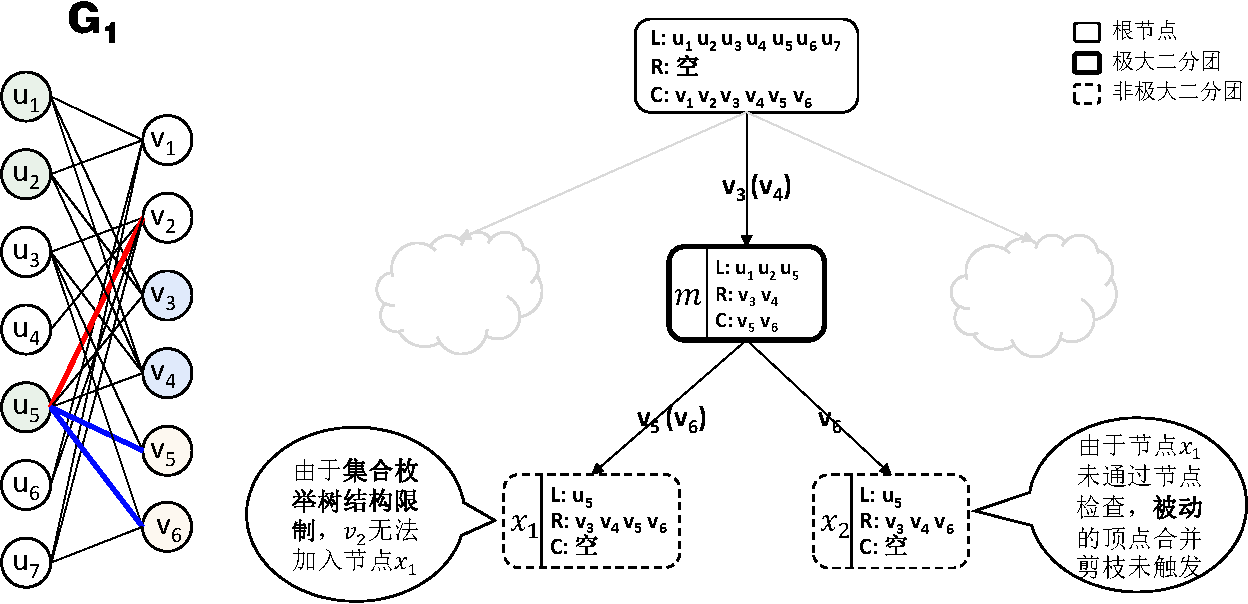
\includegraphics[width=0.9\linewidth]{ambea_motivation}
  % \vspace{0.1 in}
  \caption{二分图$G_1$上的部分集合枚举树}
  \label{fig:ambea_motivation}
\end{figure}

\begin{example}
  图~\ref{fig:ambea_motivation}是图~\ref{fig:se_mbea}的子图,展示了在二分图$G_1$上,以节点$m$为根节点的部分集合枚举树,用于说明本章研究动机。为便于观察,我们在图$G_1$中标记了节点$m$中的顶点,并标记了集合$L_m$和集合$C_m$之间的边,以及集合$L_m$和顶点$v_2$之间的边。

  在所示的部分集合枚举树中,我们观察到节点$x_1$和节点$x_2$的集合$L$都只包含顶点$u_5$,而且顶点$v_2$与顶点$u_5$相连。根据深度优先的搜索规则,顶点$v_2$在节点$x_1$和节点$x_2$生成之前已被访问。由于集合枚举树的结构限制,节点$x_1$和节点$x_2$不允许使用已访问的顶点$v_2$来扩展它们的集合$R$,从而导致非极大二分团的产生。
  同时,我们观察到在节点$m$中,候选顶点$v_5$和$v_6$在$L_m$中的邻居同是$u_5$,这意味着可以通过顶点合并对由顶点$v_6$生成的节点$x_2$进行剪枝。然而,由于顶点$v_5$生成的节点$x_1$产生了非极大二分团,被动的顶点合并剪枝方法没有被触发,因此该方法的性能没有充分发挥。

\end{example}

\section{AMBEA算法设计与实现}

为了克服现有方法的不足,本节提出了激进的集合枚举树和激进的顶点合并剪枝方法,以提升极大二分团枚举算法的效率。其中,激进的集合枚举树突破了传统集合枚举树的结构限制,而激进的顶点合并剪枝方法则有效地优化了剪枝过程。最终,我们综合应用这两种技术,形成了高效的极大二分团枚举算法AMBEA。

\subsection{激进的集合枚举树}
\label{subsec:ase}

现有基于集合枚举树的极大二分团枚举算法存在一个限制,即它们只使用未遍历的顶点来生成的树节点(二分团)以确保区分性。因此它们通常需要进行大量节点检查以消除产生的大量非极大二分团。为了克服这一限制,我们提出了一种新颖的\textbf{激进的集合枚举树}(Aggressive Set-Enumeration Tree,ASE Tree),在\textit{节点生成}过程中,它激进地引入所有顶点,将所有二分图扩展到它们的极大二分团形式,避免检查它们的极大性。考虑到这种激进的扩展可能导致生成重复的二分图,我们在\textit{节点检查}过程中通过使用低成本方法来消除重复实例并输出不同的极大二分团来解决这个问题。

% 为了确保枚举树中每个节点对应的二分团都是不同的,传统的集合枚举树在扩展每个节点的二分团时,对顶点的选择进行了结构限制。然而,我们观察到保证每个节点对应的二分团互不相同并不是解决极大二分团枚举问题的必要条件。因此,我们设计了一种激进的集合枚举树,简称为ASE树(Aggressive Set Enumeration Tree)。ASE树不再对扩展节点内的二分团顶点施加限制,并利用父子节点之间的联系设计了新的节点检查规则以确保算法的正确性,并释放额外的搜索空间优化潜力。

在展开描述之前,我们先定义一些重要的术语和符号。

\begin{definition}
  ($\vec{\mathbf{v}}$) 对于一个枚举树节点,$\vec{v}$ 表示用于生成该枚举树节点的候选顶点,即从父节点到子节点的边上的遍历候选顶点。例如,在图~\ref{fig:ambea_motivation}中,节点$m$的$\vec{v}$是$v_3$。
\end{definition}

\begin{definition}
  ($\mathbf{X_v^+, X_v^-}$) 给定顶点顺序,顶点集$X$可以被顶点$v$划分成两个子集:$X_v^+$ 包含所有顶点比 $v$ 更大的顶点(顺序在 $v$ 之后的顶点),即顶点$v$的尾部顶点;$X_v^-$ 包含包括 $v$ 顶点在内的所有顶点比 $v$ 更小的顶点(顺序在 $v$ 之前的顶点),即顶点$v$的头部顶点。
\end{definition}


具体而言,ASE树保留了传统集合枚举树的节点结构,并设计了激进的节点生成方法和节点检查方法。\textbf{节点生成的过程允许使用所有顶点来扩展新节点的二分团,因此每个节点都会产生一个极大二分团},但是不同节点对应的二分团可能重复。为了消除全部重复二分团,我们利用父子节点的联系设计了新的节点检查规则。我们对ASE树的节点生成以及节点检查规则进行了规范化描述:

% \begin{itemize}
%   \item 节点生成:ASE树从根节点$(U,\emptyset,V)$ 开始遍历。对于当前节点$(L,R,C)$,ASE树按顺序访问集合$C$中的每个候选顶点$v'$以生成一个新的节点$(L',R',C')$。集合$L'$包含集合$L$和集合$N(v')$中的共同顶点。集合$R'$包含所有与集合$L'$内顶点均相连的顶点。集合$C'$包含集合$C$中与集合$L'$内顶点部分相连的且未被访问的顶点。

%   \item 节点检查:假设当前节点$(L,R,C)$选择$v'$生成新节点$(L',R',C')$且当前节点的$\vec{v}$是$v$,新节点通过节点检查并输出一个极大二分团当且仅当满足以下全部条件:
  
%   \begin{itemize}
%     \item O1: $v$是集合$R'$内满足$\Gamma({R'}_{v}^-) \cap N(v') = L'$的最小顶点。
%     \footnote{为了方便起见,我们假设顶点可以根据预定的顺序进行比较。例如,$v_x > v_y$表明$v_x$的顺序在$v_y$之后,即$x > y$。}
%     \item O2: ${R}_{v}^-$ 和 ${R'}_{v}^-$相同。
%     \item O3: $v'$是集合$R'$内满足$\Gamma({R'}_{v'}^-) = L'$的最小顶点。
%     \item O4: 由根节点产生的节点是需要检查条件O3。
%   \end{itemize}
  
% \end{itemize}

\textbf{节点生成:}ASE树的遍历从根节点$(U, \emptyset, V)$开始,依次遍历当前节点$(L, R, C)$中的每个候选顶点$v'$,以生成新节点$(L', R', C')$。在新节点中,$L'$表示$R\cup\{v'\}$的共同邻居,即$L' = L\cap N(v')$。不同之处在于,$R'$包含$L'$中顶点的所有共同邻居,即$R' = \Gamma(L')$。$C'$由$C$中顺序在顶点$v'$之后且与集合$L'$中任意顶点相连的顶点组成,即$C'= C_{v'}^+ \cap (\Upsilon(L') - \Gamma(L'))$。

\textbf{节点检查:} 为了识别和消除上述节点生成过程中产生的所有重复的极大二分团,我们采用\textbf{基于映射的节点检查基本方法}。具体而言,我们为每个极大二分团$(L', R')$分配唯一的\emph{目标顶点} $v'_T$和唯一的\emph{目标父节点} $(L_T, R_T)$。对于目标父节点选择目标顶点所产生的节点,我们输出对应的极大二分团;对于其他节点,我们消除它们产生的重复项。映射的细节如下:

\vspace{-0.5in}
\begin{align}
	\label{eq:target_v}
	& \begin{aligned}
		\hspace{13pt} v'_T &= \min\{v \in R' \mid \Gamma({R'}_{v}^-) = L' \}
	\end{aligned} \\
	\label{eq:target_parent}
	& \left\{
	\begin{aligned}
		v_T &= \min\{v \in R' \mid \Gamma({R'}_{v}^-) \cap N(v'_T) = L'\} \\
		L_T &= \Gamma({R'}_{v_T}^-) \\
		R_T &= \Gamma(L_T)
	\end{aligned}
	\right.
\end{align}


在映射中,根据公式~\ref{eq:target_v},$v'_T$是$R'$中满足条件$\Gamma({R'}_{v}^-) = L'$的最小顶点$v$,也是仅根据极大二分团$(L', R')$能够确定的唯一目标顶点。确定了$v'_T$后,如果$N(v'_T)$与$L'$相同,则$(L_T, R_T)$为根节点;否则,$(L_T, R_T)$根据公式~\ref{eq:target_parent}确定。根据公式~\ref{eq:target_parent},我们首先得到中间顶点$v_T$,它是$R'$中满足条件$\Gamma({R'}_{v}^-) \cap N(v'_T) = L'$的最小顶点$v$,也是仅根据极大二分团$(L', R')$和$v'_T$能够得到的唯一顶点。然后,我们可以将$L_T$推导为$\Gamma({R'}_{v}^-)$,将$R_T$推导为$L_T$中顶点的共同邻居。

根据这种映射机制,节点$(L', R', C')$通过节点检查并输出极大二分团,当且仅当以下两个条件同时满足:
% 节点$(L', R', C')$仅在满足以下两个条件时输出一个极大二分团:

- O1:当前节点的$\vec{v}$是目标顶点$v'_T$。

- O2:父节点中的极大二分团是目标父节点的极大二分团$(L_T, R_T)$。

% \begin{itemize}
% 	\item O1:当前节点的$\vec{v}$是目标顶点$v'_T$。
% 	\item O2:父节点中的极大二分团是目标父节点的极大二分团$(L_T, R_T)$。
% \end{itemize}

为了提高对ASE树中重复节点的检查效率,我们引入了一种\textbf{低成本节点检查}方法。该方法无须进行多集合求并集运算,仅需访问候选顶点的局部邻居。如果子节点和父节点中同一候选顶点$v_c$对应的局部邻居保持不变(即$L_{parent} \cap N(v_c) = L_{current} \cap N(v_c)$),我们可以安全地裁剪掉子节点选择候选顶点$v_c$所生成的节点。因为根据节点生成规则,父节点和当前节点通过遍历顶点$v_c$会生成相同的二分团。根据公式~\ref{eq:target_parent},映射机制选择满足条件的最小$v_T$,即确保目标父节点的$\vec{v}$最小。由此可知当前子节点不能对应于二分图$(L_T, R_T)$,因为$|L_{current}|<|L_{parent}|$。这种低成本节点检查只需要$O(\Delta(V))$的集合交集运算,而其他方法至少需要$O(|E|)$的计算量。

与传统的搜索空间优化方法不同,ASE树彻底改变了集合枚举树的节点生成方式和节点检查方式。通过采用激进的节点生成规则,枚举树中的二分团被扩展为极大二分团,并且允许重复。同时,配套的节点检查规则确保ASE举树能够无重复地输出二分图中的全部的极大二分团。我们在理论上为基于ASE树的极大二分团枚举算法提供了\textbf{正确性证明}。


\begin{theorem}
  \label{theorem:correctness}
  ASE树能够准确的输出二分图中的全部极大二分团,并排除任何非极大二分团或重复二分团。
\end{theorem}

\begin{proof}
  首先,根据节点生成规则,对于新生成的节点$(L',R',C')$,我们可以得到$L'=L\cap N(v')=\Gamma(R\cup\{v'\})$且$R'=\Gamma(L')$。因为$L'$和$R'$都是某个特定集合内顶点的共同邻居且$R'$内的顶点和$L'$内的顶点均相连,所以$(L',R')$是一个极大二分团。由此可知,在激进的生成规则下不会产生非极大二分团。

  其次,根据节点检查规则,每个节点可以根据产生的二分团$(L',R')$计算得到唯一的\emph{目标顶点$v'_T$}和唯一的对应于极大二分团$(L_T, R_T)$的\emph{目标父节点}。对于对应于$(L_T, R_T)$的给定节点,我们知道$v'_T$总是包含在其候选集$C_T$中,因为$v'_T$始终大于$v_T$并与$L_T$中的一些但不是所有顶点相连。因此,如果目标父节点$(L_T,R_T,C_T)$存在,它总是可以通过遍历$v'_T$生成具有$(L', R')$的节点。
  
  
  % \emph{靶顶点$\vec{v}$}和唯一的\emph{靶父节点}$(L,R,C)$。我们把靶顶点$\vec{v}$记作$v'$。通过判断当前节点是否由靶父节点访问靶$\vec{v}$产生,我们可以消除重复二分团。具体而言,为了计算靶顶点$\vec{v}$,我们按照给定顺序逐个添加$R'$内的顶点初始为空的集合$X$中,直到$\Gamma(X)$等于$L'$。$v'$是最后一个添加到$X$的顶点。类似的,为了计算靶父节点$(L,R,C)$,我们按照给定顺序逐个添加$R'$内的顶点到初始为空的集合$Y$中,直到$\Gamma(Y)$和$N(v')$的交集等于$L'$。这时,我们可以得到$L=\Gamma(Y)$,$R=\Gamma(L)$。节点$(L,R,C)$的靶顶点$\vec{v}$是最后一个添加到集合$Y$中的顶点,记作$v$。因为$v'>v$并且$v'$与$L$中的部分顶点连接,所以$v'$在$C$中。
  
  最后,根据节点检查规则,通过遵循这个过程,每个极大二分团的对应节点可以递归地找到唯一的靶父节点,直到达到根节点。因此,ASE树总能够准确地无重复地枚举每个极大二分团。
\end{proof}





\begin{algorithm}[H]
  \begin{algorithmic}[1]
      \normalsize
      \REQUIRE 二分图 $G(U,V,E)$
      \ENSURE 所有极大二分团
      
      \renewcommand{\algorithmicdo}{\textbf{do}}
      \FOR{$v_s\in V$}
        \STATE \textsf{biclique\_search\_ase}$(U,\emptyset,V,v_s)$;
      \ENDFOR

      \renewcommand{\algorithmicwhile}{\textbf{procedure}}
      \renewcommand{\algorithmicdo}{\textbf{:}}
      \WHILE{\textsf{biclique\_search\_ase}$(L,R,C,v')$}
      \renewcommand{\algorithmicdo}{\textbf{do}}
      \STATE $L' \leftarrow L \cap N(v'); R' \leftarrow \Gamma(L'); C' \leftarrow \emptyset$;
      \STATE $\overline{L}\leftarrow L \setminus L'; \overline{R}\leftarrow {R'}_{v'}^- \setminus (R \cup C)$;

        \FOR{$v_c \in C$}
          \IF{$L' \cap N(v_c) = L'$}  
            \IF{$v_c < v'$}
              \STATE $\overline{L} \leftarrow \overline{L} \cap N(v_c)$; 
            \ENDIF
          \ELSIF{$L' \cap N(v_c) \neq \emptyset \land v_c > v'$}
            \STATE $C' \leftarrow C' \cup \{v_c\}$;
          \ENDIF
        \ENDFOR

        \IF{$\overline{L} \neq \emptyset \land \overline{R} = \emptyset$}
          \STATE 输出极大二分团$(L', R')$;
          \FOR{$v_c'\in C'$}
            \IF{$N(v_c') \cap \overline{L} \neq \emptyset $}
              \STATE \textsf{biclique\_search\_ase}$(L', R', C', v_c')$;
            \ENDIF
          \ENDFOR
        \ENDIF
      \ENDWHILE

  \end{algorithmic}
  \caption{基于ASE树的极大二分团枚举算法}
  \label{alg:ase}
\end{algorithm}



算法~\ref{alg:ase}总结了基于ASE树的极大二分团枚举算法的基本枚举过程。该算法依次遍历$V$中的每个顶点$v_s$,并递归地调用过程\textsf{biclique\_search\_ase}(第1-3行)。这个过程描述了节点$(L,R,C)$访问候选顶点$v'$生成节点$(L',R',C')$ (第5、12-13行)并执行节点检查的过程(第6、8-11、16行)。接下来我们概述节点检查的执行过程。我们把节点$(L,R,C)$的$\vec{v}$记作$v$。由于节点$(L,R,C)$已通过节点检查,这意味着$\Gamma(R_v^-) = L$且$v$是$R$中满足$\Gamma(R_v^-) \cap N(v') = L'$的最小顶点(第19行),因此满足条件O1。值得注意的是,ASE树支持使用简单的集合交集运算在$O(\Delta(V))$的时间复杂度内进行\textbf{低成本的节点检查},而其他节点检查方法至少需要$O(|E|)$的时间复杂度。根据节点的生成规则,由于$R \cup C$包含了所有与$L'$中的某些或全部顶点相连的比$v$大的顶点,因此我们知道$\overline{R}$中的顶点都比$v$小。如果$\overline{R} = \emptyset$ (第16行),则表示在$R'$中没有比$v$小且不在$R$中的顶点。我们使用$\overline{L}$ 来存储与$L$中的部分顶点,这部分顶点与$R'$内小于$v'$的全部顶点相连且和$v'$不相连。因此,如果$\overline{L} \neq \emptyset$ (第16行),则满足条件O2。

就时间复杂度而言,由于算法中最复杂的操作涉及最多$|V|$次集合操作且每次集合操作耗时$O(\Delta(V))$,因此ASE树中每个节点的计算时间为$O(|V|\Delta(V))$。最终,算法~\ref{alg:ase}的时间复杂度为$O(|V|\Delta(V)\beta)$,与算法~\ref{alg:se_mbe}相同。

我们用下面的例子进行详细说明。

\begin{figure} [ht]
  \vspace{0.1 in}
  \centering
  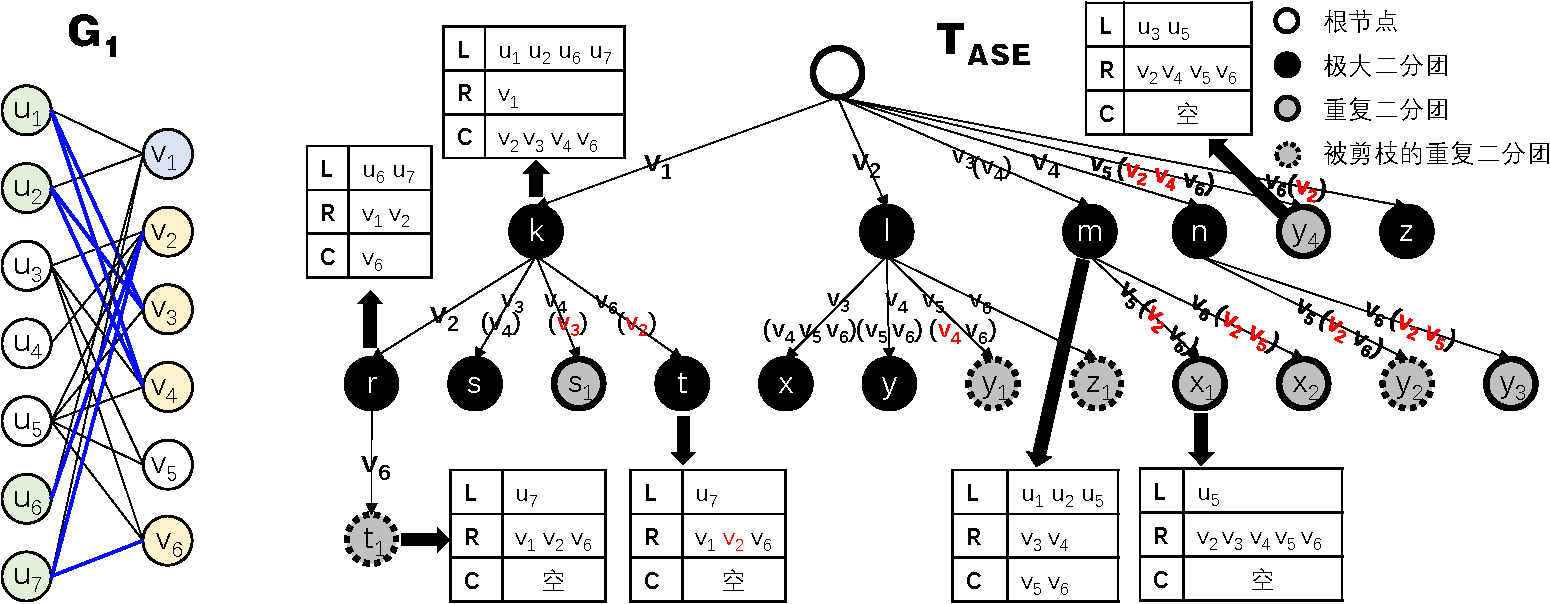
\includegraphics[width=0.98\linewidth]{eg_ase}
  % \vspace{0.1 in}
  \caption{算法~\ref{alg:ase}二分图$G_1$上的集合枚举树}
  \label{fig:ase}
\end{figure}

\begin{example}
  \label{example:ase}
  % 图~\ref{fig:ase}展示了算法~\ref{alg:ase}在二分图$G_1$上的集合枚举树$T_{ASE}$。为便于观察,我们在图$G_1$中标记了节点$k$中的顶点,并标出了集合$L_k$与集合$C_k$之间的边。ASE树和其他集合枚举树最大的区别在于ASE树允许使用所有顶点来扩展新节点的二分团,包括已访问的顶点。例如,在ASE树中,节点$k$访问$v_6$生成节点$t$的过程中,允许使用已访问的$v_2$扩展$R_t$,因此输出一个极大二分团。相反地,在图~\ref{fig:se_mbea}所示的基本的集合枚举树中,节点$k$访问$v_6$产生一个非极大二分团。

  % ASE树采用激进的节点检查规则消除重复二分团。为了更好地解释节点检查规则中的4个条件,我们用产生重复二分团的节点$t_1$, $x_1$和$y_4$举例。对于节点$t_1$,我们发现它的父节点$r$的$\vec{v}$是$v_2$。通过计算$\Gamma(\{v_1\})\cap N(v_6)=\{u_7\} = L_{t_1}$,我们得知$v_2$不是满足条件O1中等式的最小顶点,因此节点$t_1$不满足条件O1。值得注意的是,在节点$r$对应的程序到第19行时,因为$N(v_6) \cap (L_k \setminus L_r) = \{u_3, u_5, u_7\} \cap \{u_1, u_2\} = \emptyset$,所以节点$r$利用低成本的节点检查裁剪掉节点$t_1$。对于节点$x_1$,我们发现它的父节点$m$的$\vec{v}$是$v_3$。通过计算可知$v_2$在$R_{x_1}$中但不在$R_{m}$中,因此节点$x_2$不满足条件O2,即$\overline{R}\neq\emptyset$ (第16行)。对于节点$y_4$,我们发现它的$\vec{v}$是$v_5$,且它的父节点是根节点。根据条件O4,我们只需要检查条件O3。通过计算$\Gamma(\{v_2, v_4\}) = \{u_3, u_5\} = L_{y_4}$,$v_5$不是满足条件O3中等式的最小顶点,因此节点$y_4$不满足O3,即$\overline{L}=\emptyset$ (第16行)。
  
  % 相对于集合枚举树图~\ref{fig:se_mbea}中的集合枚举树$T_{SE}$,$T_{ASE}$ 能够产生相同的极大二分团。然而,$T_{ASE}$ 独具优势的地方在于,它使用低成本的节点检查方法,可以额外裁剪掉无效节点,例如$t_1, y_1, z_1$ 和$y_2$等节点,从而进一步提高算法的效率。

  图~\ref{fig:ase}展示了在二分图$G_1$上的一个枚举树$T_{ASE}$。$T_{ASE}$与图~\ref{fig:se_mbea}中的$T_{SE}$之间的主要区别在于节点生成过程。具体来说,在$T_{ASE}$中,每个节点都可以通过遍历顶点进一步扩展,如图中所示。例如,在$T_{SE}$中,当节点$k$遍历$v_6$时,它生成了一个非极大二分团的节点$t_1$,因为$T_{SE}$无法使用$v_2$扩展$R_{t_1}$,因为$v_2$已经被遍历以生成节点$r$。相比之下,在$T_{ASE}$中,节点$k$在遍历$v_6$时生成了一个极大二分团的节点$t$,因为$T_{ASE}$可以使用$v_2$扩展$R_{t}$。因此,$T_{ASE}$中的所有二分团都是极大的,但可能存在重复的二分团,比如节点$t$和节点$t_1$。

  $T_{ASE}$采用了一种激进的节点检查规则来消除重复的二分团。为了说明节点检查的条件,我们将以节点$x_1$和$t_1$为例。对于节点$x_1$,根据公式~\ref{eq:target_v},我们按顺序将顶点从$R_{x_1}$添加到空集$X$,直到$\Gamma(X)$等于$L_{x_1}$。通过这样做,我们确定节点$x_1$的$v'_T$是$v_3$,因为$\Gamma(\{v_2,v_3\}) = \{u_5\}=L_{x_1}$。因此,节点$x_1$不满足条件O1,因为它的$\vec{v}$是$v_5$,而不是$v_3$。对于节点$t_1$,我们以相同的方式得到它的$v'_T$为$v_6$。类似地,使用公式~\ref{eq:target_parent},我们推断出它的$v_T$是$v_1$,因为$\Gamma(\{v_1\}) \cap N(v_6) = \{u_7\}=L_{t_1}$。然后,我们发现它的$L_T = \Gamma(\{v_1\}) = \{u_1, u_2, u_6, u_7\}$。因此,节点$t_1$不满足条件O2,因为其父节点$r$的集合$L$(即$L_r=\{u_6, u_7\}$)与其$L_T$不相同。
  
  与$T_{SE}$相比,$T_{ASE}$输出相同的极大二分团集合。此外,$T_{ASE}$通过低成本的节点检查裁剪比$T_{SE}$更多的节点,如节点$t_1$,$y_1$,$z_1$和$y_2$。例如,节点$r$主动裁剪了节点$t_1$,因为$L_k \cap N(v_6) = \{u_7\} = L_r \cap N(v_6)$。





\end{example}

ASE树的主要贡献包括以下两点:

\begin{enumerate}
  \item \textbf{支持低成本的节点检查:}  ASE树通过支持低成本的节点检查,能够激进地裁剪无效节点,从而减小搜索空间。具体而言,在不考虑其他搜索空间优化方法的情况下,我们观察到对于$T_{SE}$和$T_{ASE}$中输出相同极大二分团$(L,R)$的节点总是具有相同的$\vec{v}$和相同候选集合$C'$,即$\vec{v}$始终对应公式~\ref{eq:target_v}中的$v'_T$,且候选集合$C'$始终是$(\Upsilon(L') - \Gamma(L'))_{v'_T}^+$。例如在图~\ref{fig:se_mbea}和图~\ref{fig:ase}中,输出相同极大二分团的节点$k$对应的$\vec{v}$均为$v_1$,且对应的候选集合均为$\{v_2,v_3,v_4,v_6\}$。由此我们知道,不同枚举树中输出相同极大二分团的节点总会产生$|C'|$个分支,对应地$T_{SE}$和$T_{ASE}$总是产生相同数量的枚举节点。因此,与基本的$T_{SE}$树相比,ASE树通过低成本的节点检查激进地裁剪无效节点,减少了需要进行节点检查过程的节点数量。
  
  % 具体而言,在不考虑其他搜索空间优化方法的情况下,$T_{SE}$和$T_{ASE}$总是产生相同数量的节点。输出相同极大二分团$(L,R)$的节点总是具有相同的$\vec{v}$和相同候选集合$C$。这是因为  两个树都确保公式~\ref{eq:target_v}中的$v'_T$始终是有效节点$(L', R', C')$的$\vec{v}$,并且候选集$C'$始终是$(\Upsilon(L') - \Gamma(L'))_{v'_T}^+$。因此,与基本的$T_{SE}$树相比,ASE树通过低成本的节点检查激进地裁剪无效节点,减少了需要进行昂贵节点检查过程的节点数量。

  \item \textbf{生成更加平衡的枚举树:} ASE树通过激进的节点生成和检查规则,倾向于降低每个枚举节点的深度,从而生成更加平衡的枚举树,有利于并行扩展。具体而言,对于不同枚举树中输出相同极大二分团$(L,R)$的节点,根据ASE树的节点检查规则O1,因为ASE树中该节点的父节点总是具有较小的$\vec{v}$,即公式~\ref{eq:target_parent}中的$v_T$,所以这些节点在ASE树中的深度更小。因此,ASE树的高度更低且更平衡。平衡的枚举树将带来相对均衡的负载,从而更有利于算法的并行扩展。

\end{enumerate}

%  ASE树通过支持低成本的节点检查,能够激进地裁剪无效节点,从而减小搜索空间。具体而言,在不考虑其他搜索空间优化方法的情况下,$T_{SE}$和$T_{ASE}$总是产生相同数量的节点。这是因为在不同的枚举树中,输出相同极大二分团$(L,R)$的节点总是具有相同的$\vec{v}$和相同候选集合$C$。其中$\vec{v}$是$R$中满足$\Gamma(R_v^-)=L$的最小顶点$v$,候选结合$C$是所有顺序在$v$之后且与$L$中某些但不是全部顶点相连的顶点集合。因此,由于ASE树额外支持低成本的节点检查,需要检查的节点数量比基本的集合枚举树更少,从而提高了计算效率。


\subsection{激进的顶点合并剪枝方法}
\label{subsec:amp}


为了进一步提升剪枝效率,我们设计了一种激进的顶点合并剪枝方法,简称AMP (Aggressive Merge-based Pruning)方法。与被动的剪枝方法不同,AMP方法通过\textbf{改变节点的生成过程,在每个节点处主动地对具有相同局部邻居的顶点进行合并},从而实现剪枝效果。此外,AMP方法具有通用性,可以应用到其他极大二分团枚举算法中,以降低节点生成过程的时间复杂度。

我们首先给出顶点局部邻居的定义,并给出顶点合并剪枝方法的理论依据。

\begin{definition}
  \textbf{(局部邻居)} 对于节点$(L,R,C)$,$C$中候选顶点$v$的局部邻居指$L$中与$v$相连的共同顶点,记作$N_L(v)$,即$N_L(v) = L \cap N(v)$。
\end{definition}

\begin{theorem}
  对于节点$(L,R,C)$,假设$v_1$和$v_2$是$C$中的两个候选顶点。如果$v_1$和$v_2$具有相同的局部邻居,那么$v_1$和$v_2$在后继节点中总是具有相同的局部邻居,因此可以被安全地合并。
  \label{theorem:merge}
\end{theorem}

\begin{proof}
  由于$v_1$和$v_2$具有相同的局部邻居,我们得到$N(v_1)\cap L = N(v_2)\cap L$。对于节点$(L,R,C)$的后继节点$(L',R',C')$,我们得到$L' \subset L$。进而,我们知道$N(v_1)\cap L' = N(v_1) \cap L \cap L' = N(v_2) \cap L \cap L' = N(v_2)\cap L'$。因此,$v_1$和$v_2$在后继节点中总是具有相同的局部邻居。
\end{proof}


% 通过这种合并,我们可以安全地裁剪由合并集合中较大的候选顶点产生的分支。相较于被动合并剪枝方法,AMP方法主动合并所有具有相同局部邻居的顶点,而无需依赖特定顶点,因此,在剪枝效率方面更加出色。
根据定理~\ref{theorem:merge}和被动顶点合并剪枝方法的启发~\cite{iMBEA14},我们发现通过主动合并具有相同局部邻居的顶点可以进一步释放剪枝潜力。具体而言,通过合并这些具有相同局部邻居的候选顶点,我们能够避免合并集合中编号较大的候选顶点产生的分支。相较于被动合并剪枝方法,主动合并方法无需依赖特定顶点,在剪枝效率方面更加出色。

然而,尽管主动合并节点内具有相同局部邻居的顶点具有提升剪枝效率的潜力,但它同时会带来一定的计算开销。一种直接的解决方法是存储所有候选顶点的局部邻居,并对它们进行两两比较。这种方法的时间复杂度为$O(|V|^2\Delta(V))$,即执行$O(|V|^2)$次比较操作,每次比较操作的时间复杂度是$O(\Delta(V))$。这种方法并不实用,因为它的复杂度超过了在每个节点上执行节点生成和节点检查的时间复杂度$O(|V|\Delta(V))$。因此,设计一种高效可行的顶点合并方法具有挑战性。

为了最小化合并开销,AMP方法修改了节点生成的过程。具体而言,假设节点$(L,R,C)$访问顶点$v'$生成新节点$(L',R',C')$。现有的方法通过逐个计算候选顶点的局部邻居来产生新的候选顶点集合$C'$。与现有方法不同,AMP方法将候选顶点集合$C$视为一个整体,并对这个整体进行划分,使具有相同局部邻居的顶点落在同一分组中。开始时,所有$C$中的顶点在同一个组内。然后,依次选择$L'$中的顶点$u_l$对每个组进行划分。通过检查组内的顶点是否与传入的$u_l$相连,每个组可以被分成两个子组。因此,具有相同局部邻居的候选顶点总是放在同一组中。最终,我们主动合并同组内的具有相同局部邻居的候选顶点。我们通过例子来说明AMP方法的执行过程。


\begin{figure} 
	\centering
	
	\subfloat[基本方法]{
			\label{subfig:no_amp}
			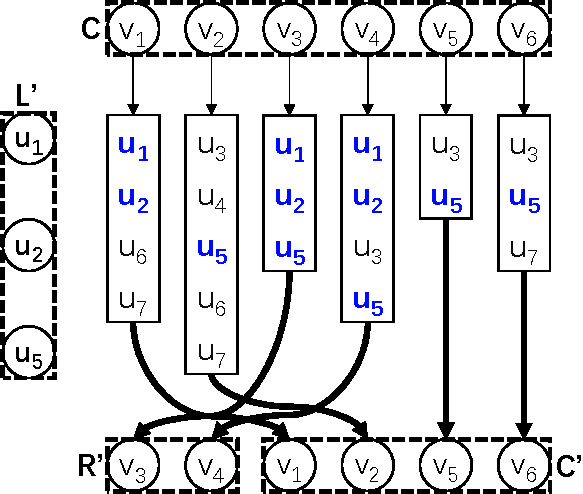
\includegraphics[width = 0.34\linewidth]{eg_no_amp}
	}
	 \quad
	\subfloat[AMP方法]{
			\label{subfig:amp}
			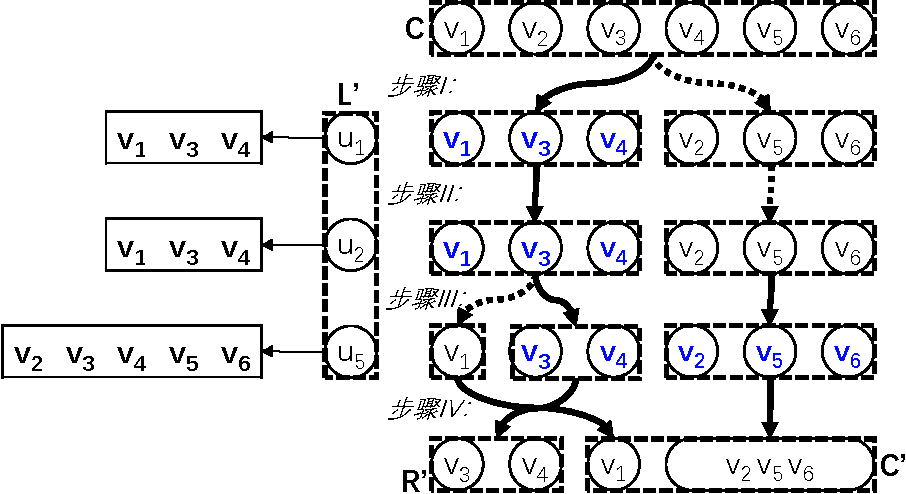
\includegraphics[width = 0.52\linewidth]{eg_amp}
	}

	\caption{图~\ref{fig:ase}中节点$m$的生成过程对比}
  \vspace{-0.05in}
	\label{fig:amp}

\end{figure}

\begin{example}
  我们用一个例子来展示AMP方法。接着例~\ref{example:ase},图~\ref{fig:amp}展示了图~\ref{fig:ase}中节点$m$在不同方法下的生成过程。为了方便比较,我们假设$C$中包含了$V$中的所有顶点。在示意图中,我们将每个顶点的邻居在矩形框中表示,并用蓝色标出了局部邻居。

  图~\ref{subfig:no_amp}展示了基本方法按顺序逐个计算候选顶点的局部邻居。而图~\ref{subfig:amp}展示了AMP方法,它使用$L'$中的顶点按顺序将候选顶点划分为多个组。  在步骤\Num1中,由于$u_1$与$v_1$、$v_3$和$v_4$相连但与其他顶点不相连,$C$被划分为两个组。在步骤\Num3中,由于$u_1$与$v_3$和$v_4$相连但与$v_1$不相连,组$\{v_1, v_3, v_4\}$被进一步划分为两个组。
在步骤\Num4中,由于$v_2$、$v_5$和$v_6$具有相同的局部邻居$\{v_5\}$,我们将这些顶点主动合并。因此,使用AMP方法,节点$m$可以裁剪由$v_5$和$v_6$生成的节点$x_1$和$x_2$。

相比之下,被动合并的剪枝方法无法裁剪节点$x_2$,因为虽然$v_5$和$v_6$具有相同的局部邻居,但由于节点$v_5$未通过节点检查,被动的顶点合并剪枝方法不会触发。

\label{example:amp}
\end{example}

\vspace{-0.2in}

\begin{figure} 
	\centering
	
  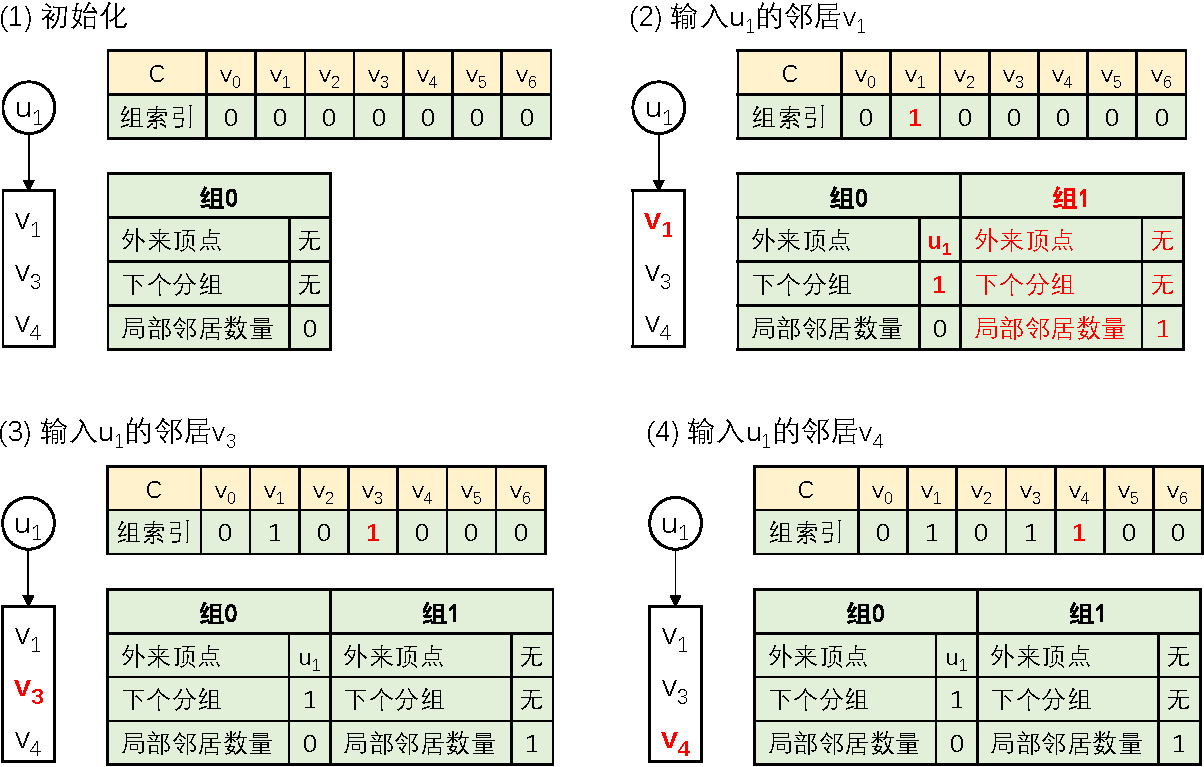
\includegraphics[width=0.85\linewidth]{eg_amp_detail}
  % \vspace{-0.05in}
	\caption{AMP方法执行组划分的详细过程}
	\label{fig:amp_detail}

\end{figure}

\begin{example}
  接着例~\ref{example:amp},图~\ref{fig:amp_detail}详细展示了AMP方法在图~\ref{subfig:amp}的步骤\Num1中进行组划分的过程。其他步骤依此类推。
  首先,我们为候选顶点集$C$中每个顶点绑定一个组索引,每个索引指向一个记录组信息的结构。组信息结构包含三个属性:外来顶点、下一个组和局部邻居数量。外来顶点和下一个组属性被用来将输入顶点分配到正确的组,局部邻居数量则记录组内所有顶点的实时局部邻居数量。具体过程如下:
  (\Num1) 在初始化时,$C$中每个顶点的组索引都被设置为0,组0中的外来顶点和下一个组都为空,局部邻居数量设置为0。
  (\Num2) 当输入$u_1$的邻居$v_1$时,我们根据$v_1$的组索引找到组0。由于组0的外来顶点不是$u_1$,我们创建了一个新的组1。组1中的外来顶点和下一个组被设置为空,而且局部邻居数量比组0多1个,因为组1中的顶点相比组0中的顶点多了$u_1$。随后,我们设置组0的外来顶点为$u_1$	​这个邻居。然后,我们将组0的外来顶点设为设置$u_1$,下一个组设为1,并将$v_1$的组索引更新为1。
  (\Num3) 当输入$u_1$的邻居$v_3$时,我们根据$v_3$的组索引找到组0,并发现组0的外来顶点是$u_1$。因此,我们将$v_3$的组索引更新为组0的下个分组,也就是组1。
  (\Num4) 同样地,在输入$u_1$的邻居$v_4$后,我们将$v_4$的组索引设置为1。
  
\end{example}





\begin{algorithm}[t]
  \begin{algorithmic}[1]
    \normalsize
    \renewcommand{\algorithmicrequire}{\textbf{数据:}}
    \REQUIRE 二分图 $G(U,V,E)$
    \renewcommand{\algorithmicrequire}{\textbf{输入:}}
    \REQUIRE 原候选顶点集$C$,新集合$L'$
    \ENSURE 顶点合并后的候选顶点集$C'$
    
    \renewcommand{\algorithmicwhile}{\textbf{struct}}
    \renewcommand{\algorithmicdo}{\textbf{:}}
    \WHILE{\textbf{GroupInfo}}
      \STATE \textbf{Integer} $incoming\_v$;
      \STATE \textbf{Integer} $next\_gid$;
      \STATE \textbf{Integer} $ln\_size$;
    \ENDWHILE


    \renewcommand{\algorithmicwhile}{\textbf{procedure}}
    \WHILE{\textsf{partition\_merge}$(C,L')$}
    \renewcommand{\algorithmicdo}{\textbf{do}}


    \STATE 给$C$中每一个顶点附加一个属性$gid=0$;
    \STATE $GroupArray$\textsf{.append}(\textbf{GroupInfo}$(\infty, \infty, 0)$ );
    \FOR{$u_l \in L'$}
      \FOR{$v_c \in C \cap N(u_l)$}
        \STATE $cid \leftarrow v_c.gid$;
        \IF{$GroupArray[cid].incoming\_v \neq u_l $}
          \STATE $new\_gid \leftarrow GroupArray$\textsf{.size()};
          \STATE $GroupArray[cid].incoming\_v \leftarrow u_l$;
          \STATE $GroupArray[cid].next\_gid \leftarrow new\_gid$;
          \STATE $GroupArray$\textsf{.append}(\textbf{GroupInfo$(\infty, \infty, GroupArray[cid].ln\_size + 1)$});
        \ENDIF
      \STATE $v_c.gid\leftarrow GroupArray[cid].next\_gid$; 
      \ENDFOR
    \ENDFOR
    \STATE $C'\leftarrow$ 合并$C$内具有相同$gid$的顶点,不包括$ln\_size$为0或$|L'|$的组;

    \ENDWHILE

  \end{algorithmic}
  \caption{\label{alg:amp}AMP方法的执行过程}
\end{algorithm}

算法~\ref{alg:amp}展示了AMP方法的主要执行过程\textsf{partition\_merge}。该过程接收原候选顶点集$C$和新集合$L'$两个输入,使用AMP方法合并具有相同局部邻居的顶点,并返回新候选顶点集合$C'$ (第6-21行)。具体而言,算法首先给$C$中每个顶点附加一个组索引属性($gid$) (第7行),用于在动态维护的组数组$GroupArray$中检索顶点的组信息$GroupInfo$ (第8行)。其中,组信息包括输入顶点($incomming\_v$)、下个分组($next\_gid$)和局部邻居数量($ln\_size$) (第1-5行)。初始时,$GroupArray$只包含一个包含所有候选顶点的组 (第8行)。然后,算法使用$L'$中的每个顶点$u_l$迭代地对候选顶点进行分组 (第9行)。对于具有相同组索引的顶点,算法将与$u_l$相连的顶点分配到新的组中 (第10-19行)。当$u_l$不是当前组的输入顶点时,算法创建一个新的组,并将其局部邻居数量增加1 (第12-17行)。为了优化内存使用,我们建议回收没有元素的组,可以使用堆栈结构实现。最后,算法合并具有相同组索引的顶点,因为它们拥有相同的局部邻居。
就时间复杂度而言,由于创建组、更新组信息等操作均能在常数时间完成,且在运行过程中访问每条边最多1次,所以过程\textsf{partition\_merge}的时间复杂度为$O(|E|)$。

AMP方法的贡献主要包括以下两点:

\begin{enumerate}
  \item \textbf{基于主动顶点合并的剪枝方法:} 与被动的剪枝方法不同,AMP方法在节点生成的同时执行,不依赖于特定的顶点,因此总是能够主动合并节点内全部具有相同局部邻居的顶点。假设集合$X$中的顶点具有相同的局部邻居,AMP方法不仅能够裁剪掉集合$X$中除最小顶点外其他顶点所产生的无效分支,而且能够合并集合$X$内所有的计算,减少重复计算,从而提升计算效率。
  
  \item \textbf{降低节点生成过程的时间复杂度:} AMP方法修改了节点生成的过程,具有降低该过程时间复杂度的潜力。具体而言,传统的节点生成过程逐个计算每个候选顶点的局部邻居,时间复杂度为$O(|V|\Delta(V))$。而AMP方法的时间复杂度为$O(|E|) =O(|V|d_{avg}(V)) < O(|V|\Delta(V))$。因此,作为一种通用方法,AMP方法可以直接用于优化现有算法的节点生成过程。

\end{enumerate}

\subsection{AMBEA算法}
\label{subsec:ambea}
  结合ASE树和AMP方法,我们设计了一种激进的极大二分团枚举算法,简称为AMBEA (Aggressive Maximal Biclique Enumeration Algorithm)。

\begin{algorithm}[H]
  \begin{algorithmic}[1]
    \normalsize
    \REQUIRE 二分图 $G(U,V,E)$
    \ENSURE 所有极大二分团
    
    \renewcommand{\algorithmicwhile}{\textbf{procedure}}
    \renewcommand{\algorithmicdo}{\textbf{:}}

    \STATE 将$V$中顶点按照邻居数量递增排序;
    \FOR {$v \in V$}
      \STATE \textsf{biclique\_search\_ambea}$(U,\emptyset,V,v)$;
    \ENDFOR

    \WHILE{\textsf{biclique\_search\_ambea}$(L,R,C,v')$}
    \renewcommand{\algorithmicdo}{\textbf{do}}
      \STATE $L' \leftarrow L \cap N(v'); R' \leftarrow \Gamma(L')$;
      \STATE $C' \leftarrow$ \textsf{partition\_merge}    $(C_{v'}^+, L')$;
      \STATE $\overline{L} \leftarrow \emptyset'; \overline{R}\leftarrow {R'}_{v'}^- \setminus (R \cup C)$;
      \FOR{$u_l \in L \setminus L'$}
        \IF{$ ({R'}_{v'}^- \setminus \{v'\}) \subseteq N(u_l)$}
          \STATE $\overline{L} \leftarrow \overline{L} \cup \{u_l\}$;
        \ENDIF
      \ENDFOR

      \IF{$\overline{L} \neq \emptyset \land \overline{R} = \emptyset$}
        \STATE 输出极大二分团$(L', R')$;
        \FOR{$v_c'\in C'$}
          \IF{$N(v_c') \cap \overline{L} \neq \emptyset $}
            \STATE \textsf{biclique\_search\_ambea}$(L', R', C', v_c')$;
          \ENDIF
        \ENDFOR
      \ENDIF
    \ENDWHILE

  \end{algorithmic}
  \caption{AMBEA算法}
  \label{alg:ambea}
\end{algorithm}

算法~\ref{alg:ambea}详细描述了AMBEA。具体而言,对于二分图$G(U,V,E)$,在~\ref{subsec:order}节所示的顶点排序方法中,AMBEA选择将$V$中顶点按照邻居数量递增排序 (第1行),因为在这种顺序下AMBEA算法性能最优。我们将通过下一节的实验证明这一结论。随后,该算法从根节点$(U,\emptyset,V)$开始,按顺序遍历$V$中的顶点$v$,并递归地调用\textsf{biclique\_search\_ambea}过程 (第2-4行)。在枚举过程中,AMBEA同时利用了ASE树中的低成本节点检查技术和AMP方法中的主动顶点合并剪枝技术。通过两种技术的有机结合,AMBEA高效地减小了计算空间,并取得了良好的计算性能。
% 该算法有效结合了ASE树中的低成本节点检查技术(第17行)以及AMP方法中的主动顶点合并剪枝技术(第7行),从而减小了大量的搜索空间并取得了良好的计算性能。
% 该算法高效地结合了算法~\ref{alg:ase} (第8-21行) 和算法~\ref{alg:amp} (第7行),从而减小了大量的搜索空间并取得了良好的计算性能。

\begin{figure} [H]
	\centering
	
  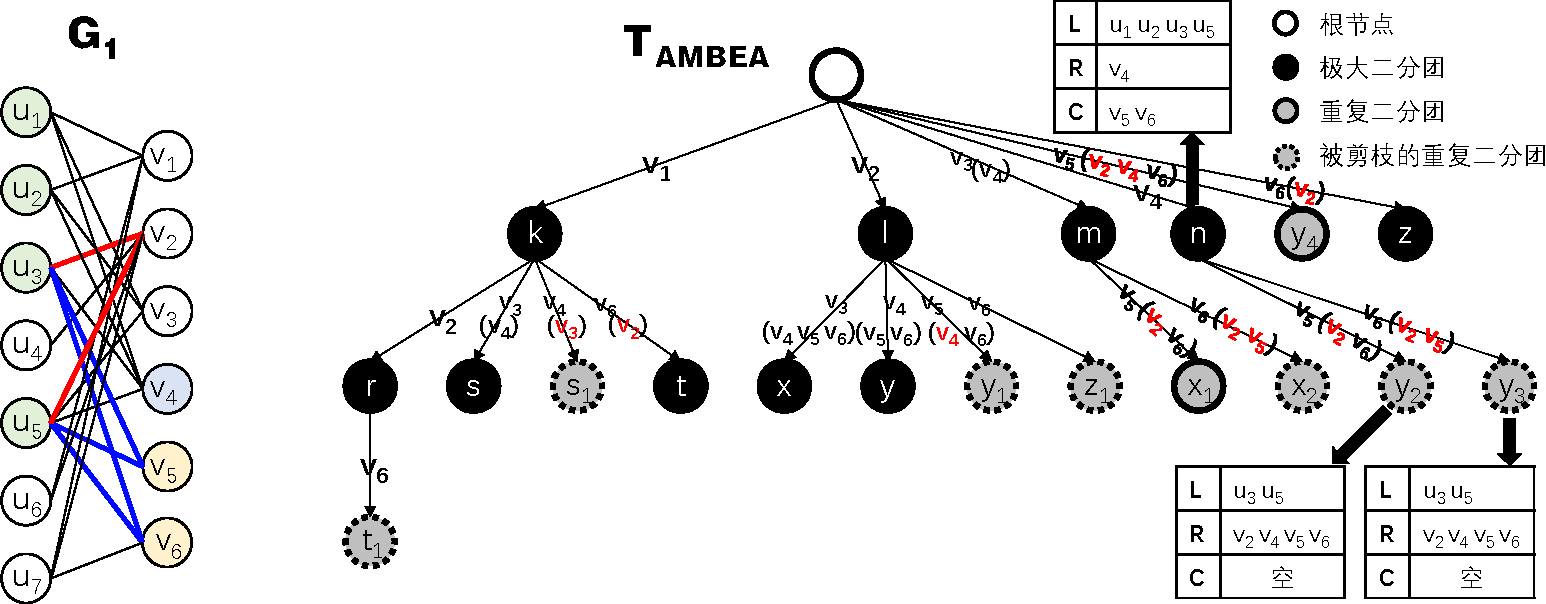
\includegraphics[width=0.98\linewidth]{eg_ambea}
  
	\caption{AMBEA在二分图$G_1$上的集合枚举树}
  \vspace{-0.1in}
	\label{fig:ambea}
\end{figure}

\begin{example}
  \label{example:ambea}
  为了方便比较,图~\ref{fig:ambea}展示了AMBEA算法在二分图$G_1$上的集合枚举树$T_{AMBEA}$时,未进行顶点排序优化的情况。为了更清晰地展示,我们在图$G_1$中标记了节点$n$中的顶点,并标出了集合$L_n$与集合$C_n$之间的边,以及集合$L_n$与顶点$v_2$之间的边。在图~\ref{fig:ase}所示的集合枚举树$T_{ASE}$的基础上,AMBEA利用AMP方法额外地裁剪节点$s_1$、$x_2$和$y_3$,充分发挥两种方法的优势。

  具体而言,当节点$r$访问候选顶点$v_5$时,因为$N(v_5) \cap (L_{root} \setminus L_r) = \{u_3, u_5\} \cap \{u_4, u_6, u_7\} = \emptyset$,所以节点$r$可以利用ASE树中所支持的低成本节点检查裁剪掉$v_5$对应的节点$y_2$。同时,由于$v_5$和$v_6$具有相同的局部邻居,算法利用AMP方法将将它们合并,并裁剪掉$v_6$对应的节点$y_3$。因此,算法能够裁剪掉节点$n$的所有无效子节点。然而,由于现有的剪枝方法只能在访问特定候选顶点后被动执行,因此无法裁剪掉节点$m$的所有无效子节点,从而限制了剪枝效率的提升。
\end{example}

结合算法~\ref{alg:ambea},我们从时间复杂度和空间复杂度两个方面对AMBEA进行分析。

\textbf{时间复杂度:} AMBEA的时间复杂度可以分为两部分,即顶点排序时间(第1行)和集合枚举树生成时间(第2-4行)。顶点排序时间复杂度为$O(|V|log(|V|))$。在每个枚举节点的计算过程中,由于$L', R', C',\overline{L},\overline{R}$ 的计算都可以通过之访问二分图中的每条边一次来得到,因此每个节点的计算复杂度为$O(|E|)$。为了量化算法的计算时间,我们沿用~\ref{subsec:baseline_analysis}节中的相关定义,用$\beta$来表示枚举树中节点的数量,包括输出极大二分团的节点和产生重复二分团的节点。由此可知,AMBEA的时间复杂度为$O(|E|\beta + |V|log(|V|))$。由于排序开销通常远小于生成集合枚举树的开销,因此,AMBEA的时间复杂度可以简化为$O(|E|\beta)$。

就每个节点的计算复杂度而言,AMBEA算法中每个节点的计算时间与ooMBEA算法相同 (即$O(|E|)$),且优于其他相关算法(即$O(|V|\Delta(V))$)。就算法的枚举空间$\beta$而言,经过~\ref{subsec:ambea_exp_overall}节的实验结果验证,AMBEA算法的枚举空间小于其他对比对象。这得益于AMBEA算法高效的剪枝能力。


\textbf{空间复杂度: } AMBEA的空间复杂度同样分为两个部分,即输入二分图所占用的空间和极大二分团枚举过程所需要的空间。输入二分图所占用的空间为$O(|E|)$。在枚举过程中,每个计算节点所需的空间为$O(|L|+|R|+|C|+|\overline{L}| + |\overline{R}|) = O(\Delta(V) + |V|) = O(|V|)$。由于枚举树的高度上界为$O(\Delta(V))$,我们可以得到AMBEA的空间复杂度为$O(|E|+|V|\Delta(V))$,与其他现有算法相同。此外,由于ASE树倾向于产生更加平衡的枚举树,因此AMBEA算法具有节省空间开销的潜力。

\textbf{并行扩展:}为了进一步提高效率,在算法AMBEA的基础上,我们开发了其并行版本ParAMBEA。受到并行算法ParMBE~\cite{parMBE19}的启发,ParAMBEA同时执行多个AMBEA中的\textsf{biclique\_search\_ambea}过程,并利用多线程优化过程内部的并行运算部分。按照算法~\ref{alg:ambea}的描述,ParAMBEA为二分图集合$V$中的每个顶点$v$分配一个线程,负责执行相应的过程 (第2-4行),即每个线程对应枚举树中由一个顶点$v$产生的子枚举树。此外,只要有多余的线程可用,ParAMBEA会动态创建子过程 (第18行)。为了最大限度地发挥并行计算资源的作用,ParAMBEA采用循环展开技术,对\textsf{biclique\_search\_ambea}过程中的所有for循环(如第9-13行、16-20行)进行并行化处理。此外,根据~\ref{subsec:ase}节的讨论,由于ASE树更倾向于生成平衡的枚举树,因此每个线程对应的负载也更加均衡,从而使ParAMBEA具有更佳的并行性能。


\section{实验评估}

本节同时使用真实数据集和合成数据集,通过与现有方法的对比对AMBEA的性能进行全面评估。首先介绍实验的环境设置,包括实验平台、数据集和比较对象。随后,通过已有算法在真实数据上的执行情况,从运行时间、剪枝效率和内存开销三个方面对AMBEA进行整体评估。接着,通过消融实验,对本章提出的ASE、AMP以及顶点排序等技术点进行分解评估。最后,对枚举树的平衡性、AMBEA算法的并行性和扩展性进行敏感性测试。

\subsection{实验设置}

\textbf{实验环境设置:} 本节的全部实验均在一台配备有4个Intel Xeon(R) Gold 5318Y 2.10GHz CPU和128GB内存的服务器上完成,其中每个CPU拥有24个计算核心,服务器共计96个计算核心。本次实验环境的操作系统为Linux kernel-5.4.0。在没有特殊说明的情况下,算法默认使用单个计算核心串行执行。

\textbf{比较算法:} AMBEA的主要比较算法是目前5个最先进的基于集合枚举树的极大二分团枚举算法,包括MBEA~\cite{iMBEA14}、iMBEA~\cite{iMBEA14}、FMBE~\cite{parMBE19}、PMBE~\cite{PMBE20}以及ooMBEA~\cite{ooMBE22}。此外,在并行性的敏感分析中,我们还将AMBEA的并行版本ParAMBEA与最先进的并行极大二分团枚举算法ParMBE进行比较~\cite{parMBE19}。我们获取到了所有对比对象的源代码。为了公平比较,我们在一个统一的框架下重新实现并优化了算法MBEA、iMBEA、FMBE和PMBE的C++代码,并基于此框架实现了AMBEA和ParAMBEA算法。由于ooMBEA和ParMBE算法的源代码已深度优化,我们没有重新实现这两个算法。此外,为了深入评估本章提到的技术点,我们实现了一些算法变体,并在对应实验中详细描述。

\begin{table} [t]
	\centering    
	\setlength{\abovecaptionskip}{0cm}  
  \setlength{\belowcaptionskip}{-0.2cm}
	\caption{AMBEA实验数据集统计信息}      
	\label{tbl:datasets}
	\setlength{\tabcolsep}{1pt}
	\begin{center}
				\normalsize{
		\begin{tabular}{|c|c|c|c|c|c|c|}
			\hline 
			\textbf{数据集} &\textbf{目录} &\textbf{类型} & \textbf{$|U(G)|$} & \textbf{$|V(G)|$} & \textbf{$|E(G)|$} &\textbf{极大二分团}\\
			\hline
			Unicode (UL) & 特征关系 & 国家-使用-语言 &  614 & 254 & 1,255 & 460\\
			UCforum (UF) & 交互关系 & 用户-发布-论坛 & 899 & 522 & 7,089 & 16,261\\
			% Wikinews & 作者关系  & 用户-编辑-文章 & 41,747  & 1,572 & 109,218 & 44,444\\
			%Writers (WR) & 作者关系 & 作者-出版-作品 & 89,355 & 46,213 & 144,340 & 57,222\\ 
			MovieLens (Mti) & 特征关系 & 标签-属于-电影 & 16,528 & 7,601 & 71,154 & 140,266\\ 
			Teams (TM) & 归属关系 & 队员-属于-团队 & 901,130 & 34,461 & 1,366,466 & 517,943 \\
			ActorMovies (AM) & 归属关系 & 电影-出演-演员 & 383,640 & 127,823 & 1,470,404 & 1,075,444\\ 
			Wikipedia (WC) & 特征关系 & 文章-属于-目录 &1,853,493 & 182,947 & 3,795,796 & 1,677,522 \\
      YouTube (YG) & 归属关系 & 用户-属于-群组 & 94,238 & 30,087 & 293,360 & 1,826,587\\  
			StackOverflow (SO) & 评分关系 & 作者-收藏-帖子 & 545,195 & 96,680 & 1,301,942 & 3,320,824 \\
			DBLP (Pa) & 作者关系 & 作者-出版-作品 & 5,624,219 & 1,953,085 & 12,282,059 & 4,899,032\\
			IMDB (IM) & 归属关系 & 电影-出演-演员 & 896,302 & 303,617 & 3,782,463 & 5,160,061\\
			BookCrossing (BX) & 交互关系 & 用户-打分-书籍  & 340,523 & 105,278 & 1,149,739 & 54,458,953 \\
			Github (GH) & 作者关系 & 用户-参与-工程 & 120,867 & 56,519 & 440,237 & 55,346,398 \\ 
			\hline
			LJ5 & 归属关系 & 用户-属于-群组& 1,837,928 & 853,994 & 5,610,437 & 2,181,295 \\
			LJ10 & 归属关系 & 用户-属于-群组& 2,301,031 & 1,421,088 & 11,227,130 & 7,430,705 \\
			LJ15 & 归属关系 & 用户-属于-群组& 2,548,619 & 1,912,139 & 16,843,216 & 22,727,251 \\
			LJ20 & 归属关系 & 用户-属于-群组& 2,704,651 & 2,357,485 & 22,456,757 & 61,836,924 \\
			LJ25 & 归属关系 & 用户-属于-群组& 2,812,080 & 2,771,510 & 28,068,423 & 151,468,807 \\

			% LiveJournal & 归属关系 & 用户-属于-群组 & 7,489,073 & 3,201,203 & 112,307,385 & -\\
			% WebTrackers & Hyperlink & Domain-Inclusion-Tracker & 27,665,730 & 12,756,244 & 140,613,762 & -\\ 
			\hline
		\end{tabular}
				}
	\end{center}
	\vspace{-0.1in}
\end{table}
 

\textbf{数据集:} 为准确评估本章提出的技术,我们同时使用了真实数据集和合成数据集。表~\ref{tbl:datasets}详细展示了实验数据集的统计信息。真实数据集来源于KONECT仓库~\cite{konect},涵盖了不同的应用场景。上半部分的表格显示了真实数据集。而下半部分的表格展示了合成数据集,这些数据集是在大数据集LiveJournal ($|U|$=7,489,073, $|V|$=3,201,203, $|E|$=112,307,385)上分别采样5\%、10\%、15\%、20\%和25\%的边所生成,记作LJ5、LJ10、LJ15、LJ20和LJ25。大数据集LiveJournal也来自于KONECT仓库。考虑到极大二分团枚举算法的运行时间与二分图中极大二分团的数量相关,因此我们按照极大二分团的数量对数据集进行了升序排列。

\subsection{整体评估}
\label{subsec:ambea_exp_overall}

我们使用三个指标对每个极大二分团枚举算法在12个真实数据集上进行整体评估:运行时间、内存使用和剪枝效率。为了保证公平性,我们为每个算法开辟一个单独的进程独立运行。测量的运行时间是进程中极大二分团枚举过程的运行时间,不包括从磁盘中加载二分图的时间。测量的内存使用是进程的最大内存使用情况。为了测量剪枝效率,我们记录了每个极大二分团算法中产生的二分团总数量$\beta$,即节点检查次数。由于给定的二分图中极大二分团的数量$\alpha$是固定的,我们可以得到算法产生的无效二分团的数量$\delta=\beta-\alpha$。因此,我们用比值$\delta/\alpha$来衡量不同算法的剪枝效率,比值越小表示剪枝效果越明显。

\begin{figure} [H]
  \centering
  \vspace{0.1in}
  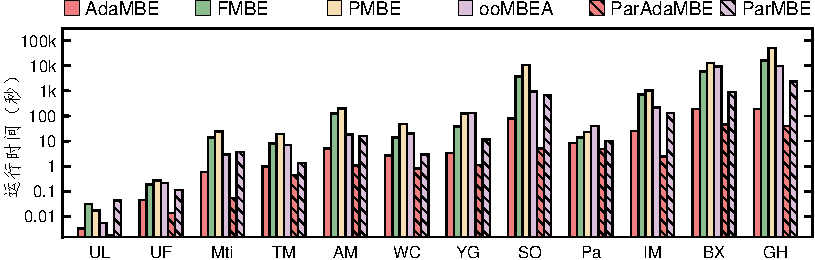
\includegraphics[width=\linewidth]{ambea/overall_time}
  \caption{AMBEA整体运行时间评估 (对数形式)}
  \label{fig:ambea_overall_time}
\end{figure}


图~\ref{fig:ambea_overall_time}展示了在真实数据集上,AMBEA与主流的极大二分团枚举算法的运行时间对比。实验结果显示,现有的极大二分团枚举算法在不同数据集上表现存在显著差异,这表明单一的极大二分团枚举算法难以满足在不同场景下的枚举性能需求。以StackOverflow、IMDB和Github等数据集为例,ooMBEA算法明显优于MBEA、iMBEA、FMBE和PMBE算法;然而,在Wikipedia、YouTube、DBLP和BookCrossing等包含大量极大二分团的数据集上,FMBE算法具有明显优势,比ooMBEA算法快1.44-3.43倍。相较于其他算法,本章提出的AMBEA算法在所有测试数据集上都展现出最短的运行时间。具体而言,AMBEA算法在各数据集上始终比最接近的其他算法快1.15-5.32倍。特别是在BookCrossing数据集上,AMBEA仅需1,609秒即可完成极大二分团枚举,而MBEA、iMBEA、FMBE、PMBE和ooMBEA算法分别需要96,206、39,036、5,934、13,234和9,452秒,这清晰地表明了AMBEA在处理耗时较长数据集时的高效率。通过结合ASE树与AMP方法的剪枝优势,AMBEA算法实现了高效的极大二分团枚举,从而在性能上超越了其他算法。


\begin{figure} [H]
  \centering
  \vspace{0.1in}
  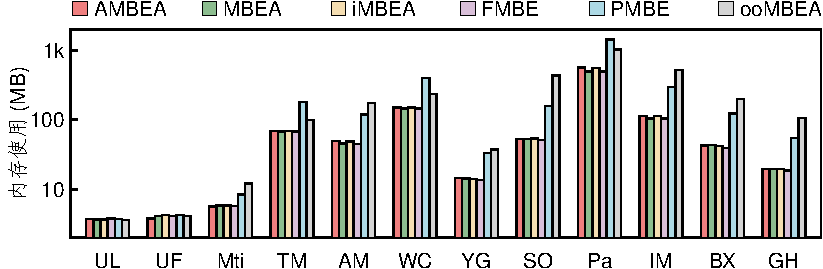
\includegraphics[width=\linewidth]{ambea/overall_memory}
  \caption{AMBEA整体内存使用评估 (对数形式)}
  \label{fig:ambea_overall_memory}
\end{figure}


图~\ref{fig:ambea_overall_memory}展示了在真实数据集上,AMBEA与主流极大二分团枚举算法的内存使用对比。实验结果显示,在所有数据集上,AMBEA、MBEA、iMBEA和FMBE的内存使用情况相当,而PMBE和ooMBEA算法则明显需要更多的内存。以StackOverflow数据集为例,AMBEA、MBEA、iMBEA和FMBE的内存使用量均为53MB、53MB、53MB和51MB,而PMBE和ooMBEA的内存使用分别高达157MB和433MB。其中,PMBE算法在初始化过程中需要额外的内存来存储CDAG索引结构,而ooMBEA算法在计算过程中将整个二分图划分为多个子二分图,因此需要额外的内存来存放这些子二分图。
从实验结果可以看出,我们提出的AMBEA算法相较于现有算法不会增加额外的内存开销。相反地,由于ASE树倾向于生成相对平衡的枚举树,这使得AMBEA在UCforum数据集上表现出最少的内存使用。由此可知,AMBEA算法在保持高效性能的同时,能够更好地控制内存资源的利用,为处理大规模数据集提供了可行的解决方案。


\begin{figure} [H]
  \centering
  \vspace{0.1in}
  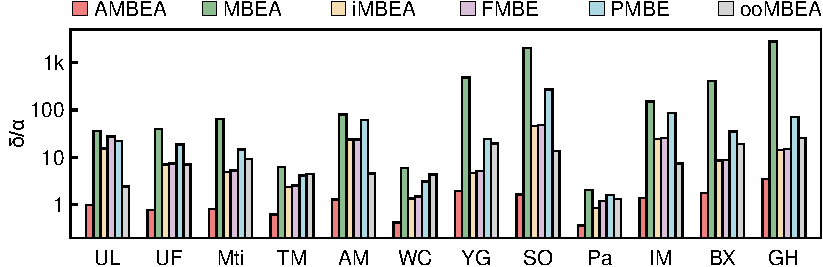
\includegraphics[width=\linewidth]{ambea/overall_prune}
  \caption{AMBEA整体剪枝效率评估 (对数形式)}
  \label{fig:ambea_overall_prune}
\end{figure}



图~\ref{fig:ambea_overall_prune}展示了在真实数据集上,AMBEA与主流的极大二分团枚举算法的剪枝效率对比。实验结果验证了本章的研究动机,即现有算法在枚举过程中所产生的搜索空间中仍然包含大量的无效二分团,并对相应节点进行节点检查,导致高昂的计算开销,正如~\ref{sec:ambea_motivation}节所讨论的。以Github数据集为例,MBEA、iMBEA、FMBE、PMBE和ooMBEA在枚举过程中分别会产生比极大二分团数量多2779.2倍、14.5倍、14.9倍、70.8倍和25.7倍的无效二分团。相应地,这些算法会通过大量高开销的节点检查过程来消除这些无效二分团,从而带来巨大的性能开销。与其他算法相比,在Github数据集上,本文提出的AMBEA算法生成的无效二分团数量仅为极大二分团数量的3.5倍,有效地压缩了搜索空间。在不同数据集上,AMBEA算法的比值$\delta/\alpha$比其他最接近的算法减少2.37-8.98倍,这意味着现有剪枝性能最优的算法产生的无效二分团数量是AMBEA中无效二分团数量的2.37-8.98倍。由此可见,AMBEA算法中高效的剪枝方法是其比其他算法更快的关键原因。




% 所有现有算法在枚举过程中会产生比极大二分团数量多15.58倍的无效二分团。对相应节点进行节点检查带来了巨大的计算开销。与其他算法相比,本章提出的AMBEA算法生成的无效二分团数量最少。在不同数据集上,AMBEA算法的比值$\delta/\alpha$比其他最接近的算法减少2.37-8.98倍,这意味着现有剪枝性能最优的算法产生的无效二分团数量是AMBEA中无效二分团数量的2.37-8.98倍。由此可见,AMBEA算法中高效的剪枝方法是其比其他算法更快的关键原因。



\subsection{技术点分解评估}

我们设计消融实验,沿用整体评估中的运行时间和剪枝效率指标。具体而言,我们在8个极大二分团数量较多的真实数据集上,对ASE树、AMP方法以及顶点排序方法进行技术点分解评估。


\begin{figure} [t]
	\centering
  % \vspace{0.05in}
	\subfloat[运行时间评估 (对数形式)]{
		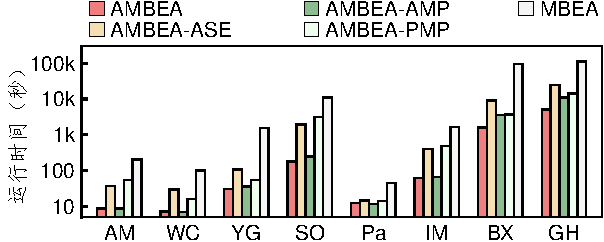
\includegraphics[width=0.7\linewidth]{ambea/time_opt}
		\label{fig:ambea_opt_time}
	}
  \vspace{0.05in}
  \\
	\subfloat[剪枝效率评估 (对数形式)]{
		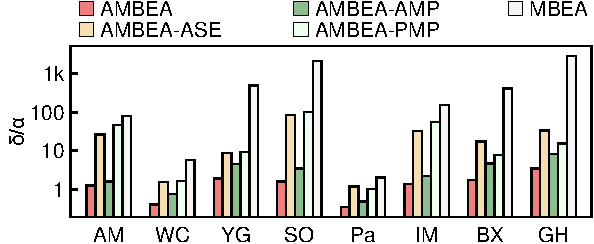
\includegraphics[width=0.7\linewidth]{ambea/prune_opt}
		\label{fig:ambea_opt_prune}
	}
  \vspace{0.05in}
	\caption{ASE树、AMP方法的技术点分解评估}
	\label{fig:ambea_opt}
\end{figure}


% \begin{figure} [H]
%   \centering
%   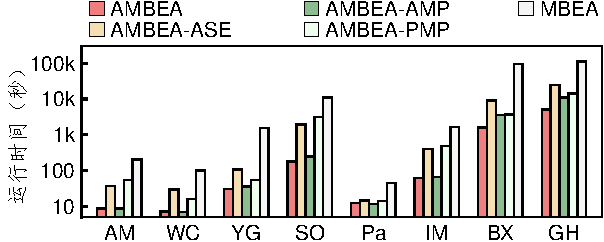
\includegraphics[width=0.75\linewidth]{ambea/time_opt}
%   \caption{细分运行时间评估 (对数形式)}
%   \label{fig:ambea_opt_time}
% \end{figure}

% \begin{figure} [H]
%   \centering
%   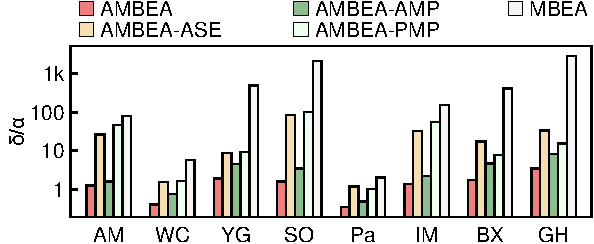
\includegraphics[width=0.75\linewidth]{ambea/prune_opt}
%   \caption{细分剪枝效率评估 (对数形式)}
%   \label{fig:ambea_opt_prune}
% \end{figure}

\textbf{ASE树的效果:}为了分解评估~\ref{subsec:ase}节提出的激进的集合枚举树技术,我们在算法MBEA~\cite{iMBEA14}的基础上应用了该技术,形成了AMBEA-ASE算法。我们选择使用MBEA算法作为基础,因为它严格按照算法~\ref{alg:se_mbe}执行,并且没有进行其他优化。如图~\ref{fig:ambea_opt}所示,AMBEA-ASE的运行时间和$\delta/\alpha$的值在所有数据集上均小于MBEA。具体而言,以YouTube数据集为例,AMBEA-ASE的运行时间是106.5秒,$\delta/\alpha$的值为1.96;而MBEA的运行时间是1,566.8秒,$\delta/\alpha$的值为484.7。由此可见,AMBEA-ASE裁剪掉了MBEA算法中$(484.7-1.96)/484.7=98.2\%$的无效二分团,并因此带来$1,566.8/106.5=14.7$倍的性能提升。这是因为在ASE树中引入了低成本节点检查技术,可以裁剪掉大量无效节点,有效的降低$\delta$的值,并且带来性能提升。

\textbf{AMP方法的效果:}为了对~\ref{subsec:amp}节提出的激进的顶点合并剪枝方法进行更详细的评估,我们设计了两个算法变体:AMBEA-AMP和AMBEA-PMP。其中,AMBEA-AMP在MBEA算法的基础上引入了激进的顶点合并剪枝方法,而AMBEA-PMP则采用了~\ref{subsec:pmp}节中介绍的被动顶点合并剪枝方法(Passive Merge-based Pruning, PMP)。如图~\ref{fig:ambea_opt}所示,与MBEA相比,AMBEA-AMP和AMBEA-PMP通过顶点合并技术裁剪了大量无效节点,在所有数据集上都取得了性能提升。此外,AMBEA-AMP的运行时间和剪枝效率一直优于AMBEA-PMP。具体来说,在StackOverflow数据集上,MBEA、AMBEA-AMP和AMBEA-PMP的$\delta/\alpha$比值分别为2,056.6,3.5和100.1。这说明AMBEA-AMP相较于AMBEA-PMP额外裁剪了96.5\%的无效二分团。因此,相较于AMBEA-PMP,AMBEA-AMP的执行时间从3,097秒缩短至248秒,带来了12.5倍的性能提升。这是因为PMP方法只有在特定顶点生成的极大二分团通过节点检测后才会合并具有相同局部邻居顶点,而AMP方法则始终激进地合并具有相同局部邻居顶点,因此带来了额外的剪枝效果。

\begin{figure} [H]
	\centering

		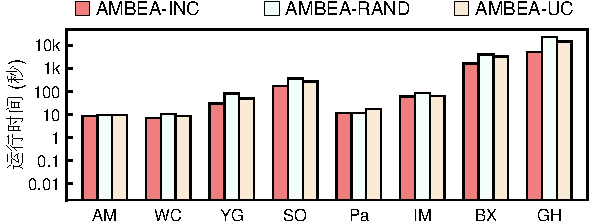
\includegraphics[width=0.7\linewidth]{ambea/order}


	\caption{顶点排序方法的分解评估(对数形式)}
	\label{fig:ambea_opt_order}
\end{figure}

\textbf{顶点排序方法的效果:}为了分解评估~\ref{subsec:ambea}节提到的按照顶点邻居数量递增排序的顶点排序方法,我们设计了三个算法变体:AMBEA-INC,AMBEA-RAND,AMBEA-UC。这三个变体均构建在AMBEA算法的基础上,唯一的区别在于集合$V$中顶点的排序方式不同。其中,AMBEA-INC按照顶点邻居数量递增排序,AMBEA-RAND不进行任何排序,而AMBEA-UC则采用单边排序方式~\cite{ooMBE22},这种方式在~\ref{subsec:order}节中已详细介绍。
如图~\ref{fig:ambea_opt_order}所示,AMBEA-INC的运行时间始终小于AMBEA-RAND和AMBEA-UC,特别是在具有许多极大二分团的数据集上表现更为明显。具体来说,在Github数据集上,AMBEA-INC的运行时间仅为5,085秒,而AMBEA-RAND和AMBEA-UC分别需要23,067秒和14,500秒。由此可见,按照顶点邻居数量递增排序的方法对于处理执行时间较长的数据集至关重要。因此,在我们的实验中,始终按照顶点邻居数量递增排序集合$V$中的顶点。


\subsection{敏感性测试}

我们对ASE树的平衡性、AMBEA算法的扩展性和并行性进行了敏感性测试。

\begin{figure} [t]
	\centering
	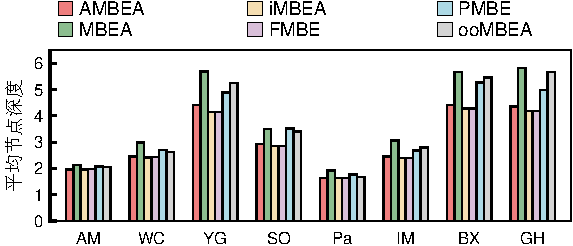
\includegraphics[width=0.7\linewidth]{ambea/balance}
	\caption{枚举树平衡性敏感性分析}
	\label{fig:ambea_exp_balance}
\end{figure}

\textbf{ASE树对枚举树平衡性的影响:}为了探索AMBEA对枚举树平衡性的影响,我们测量了不同算法生成的枚举树中每个节点的深度,并计算得到输出最大二分团节点的平均深度,具体结果见图~\ref{fig:ambea_exp_balance}。由于AMP方法不会影响输出极大二分团的节点的生成过程,因此AMBEA的平均节点深度与基本ASE树中的平均节点深度相同。我们观察到,与MBEA相比,AMBEA的平均节点深度始终更小,这说明ASE树相对于基本集合枚举树更加平衡。PMBE和ooMBEA通常具有较大的平均节点深度,这是因为它们使用了~\ref{subsec:pivot}节中提到的基于枢纽顶点的剪枝方法。具体而言,枢纽顶点$v^*$会导致满足$N_L(v')\subset N_L(v^*)$条件的顶点$v'$在当前节点不产生新节点,进而加深了顶点$v'$产生新节点的深度,导致生成的枚举树更加不平衡。iMBEA和FMBE通过在每个节点进行顶点重排序来生成平衡的枚举树。然而,在每个节点进行顶点重排序会增加额外的计算开销。总而言之,算法的选择显著影响枚举树的平衡性,与其他极大二分团枚举算法相比,AMBEA生成了相对平衡的集合枚举树,这验证了~\ref{subsec:ase}节中有关ASE树平衡性的观点。

\begin{figure} [H]
	\centering
	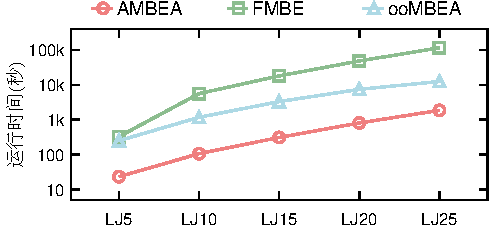
\includegraphics[width=0.7\linewidth]{ambea/scalability}
	\caption{算法扩展性敏感性分析 (对数形式)}
	\label{fig:ambea_exp_scalability}
\end{figure}

\textbf{可扩展性评估:}为了探索AMBEA的可扩展性,我们选择了FMBE和ooMBEA作为对比算法,因为它们在整体性能实验中在大规模数据集上表现出色。如图~\ref{fig:ambea_exp_scalability}所示,实验结果表明,尽管随着数据集规模的增加,不同算法的运行时间呈指数级增加,但是AMBEA算法始终在大规模合成数据集上表现出比现有方法更好的性能。具体而言,AMBEA算法在大规模合成数据集上的运行速度比FMBE快47.2倍至141.7倍,比ooMBEA快6.7倍至11.1倍。特别是在LJ25数据集上,AMBEA算法的完成时间为1,870秒,而FMBE和ooMBEA分别需要116,582秒和12,614秒。从实验结果可以看出,AMBEA算法具有良好的可扩展性,在处理大规模数据集时显示出明显的优势。


\begin{figure} [H]
	\centering
	\subfloat[StackOverflow]{
		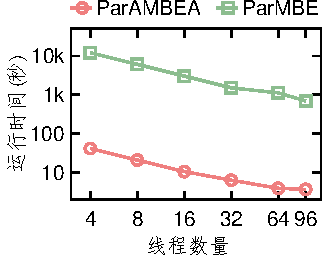
\includegraphics[width=0.4\linewidth]{ambea/parallel_so}
		\label{fig:ambea_paral_so}
	}
  \quad
	\subfloat[IMDB]{
		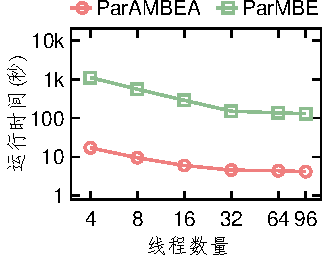
\includegraphics[width=0.4\linewidth]{ambea/parallel_im}
		\label{fig:ambea_paral_im}
	}
  \\
	\subfloat[BookCrossing]{
		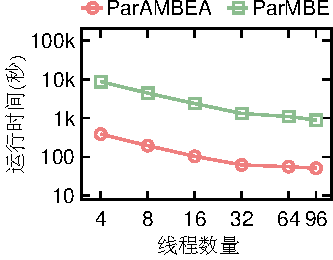
\includegraphics[width=0.4\linewidth]{ambea/parallel_bx}
		\label{fig:ambea_paral_bx}
	}
  \quad
	\subfloat[Github]{
		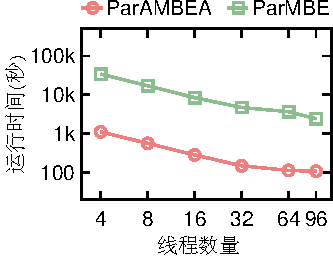
\includegraphics[width=0.4\linewidth]{ambea/parallel_gh}
		\label{fig:ambea_paral_gh}
	}
  

	\caption{算法并行性敏感性分析 (对数形式)}
	\label{fig:ambea_paral}
\end{figure}

\textbf{并行性评估:}为了探索AMBEA的并行性,我们将其并行版本ParAMBEA与最先进的并行算法ParMBE进行比较。我们在四个运行时间最长的数据集上进行了实验:StackOverflow、IMDB、BookCrossing和Github。我们分别使用4、8、16、32、64、96个线程在不同数据集上分别运行ParAMBEA和ParMBE算法。由于实验服务器中共包含96个计算核,我们将线程数量上限设置为 96。如图~\ref{fig:ambea_paral}所示,ParAMBEA 相较于 ParMBE 具有明显的性能优势,运行时间缩短了 17.4-293.8 倍。同时,从图表中我们可以观察到,随着线程数量的增加,ParAMBEA 的运行时间几乎呈线性下降趋势,这意味着它可以有效地利用更多的计算资源来加速算法的执行。值得注意的是,通过并行化,我们将 BookCrossing 数据集上 AMBEA 算法的运行时间从 1,610 秒大幅缩短至仅需 51 秒。这个结果充分证明了ParAMBEA 在并行性能方面的优越性,并显示出其在大规模数据集上的应用潜力。

\section{本章小结}

本章提出了激进的集合枚举树(ASE树)和激进的顶点合并剪枝(AMP)两种剪枝优化方法,并结合两种方法形成高效的极大二分团枚举算法AMBEA,旨在解决极大二分团问题中搜索空间大的挑战。首先,针对现有集合枚举树的局限性,即只允许使用部分顶点扩充枚举节点内二分团的结构限制,ASE树允许使用全部顶点扩展二分团,从而释放剪枝潜力,并生成更加平衡的集合枚举树。其次,针对现有剪枝方法的依赖特定顶点被动执行的问题,AMP方法通过修改节点生成过程,以较小的成本主动合并具有相同局部邻居的顶点,同时提供了降低节点生成过程时间复杂度的新思路。最后,我们将上述两种技术整合,实现了 AMBEA 算法及其并行版本 ParAMBEA。实验结果充分证明了AMBEA算法的高性能以及本章中所有剪枝方法的具体作用。
